
\subsection{Punto 1}

\textbf{Enunciado}: 

\textsl{Calcular las tensiones de todos los nodos y las corrientes de todas la ramas para $V_{G} = 0 \si[per-mode=symbol]{\volt}$.}


\vspace{1.5cm}


Se explica en detalle en \sectref{section:modelo_operacional}.



\subsection{Punto 2}

\textbf{Enunciado}: 

\textsl{Calcular la ganancia de lazo para frecuencias medias ($1 \si[per-mode=symbol]{\kilo\hertz}$).}


\vspace{1.5cm}


\textcolor{red}{\textbf{COMPLETAR!!}}



\clearpage


\subsection{Punto 3}
\label{global_gain}
\textbf{Enunciado}: 

\textsl{Calcular la ganancia global para frecuencias medias ($1 \si[per-mode=symbol]{\kilo\hertz}$).}

\vspace{1.5cm}

La ganancia global del amplificador, por tratarse de un circuito realimentado, tomando los valores calculados anteriormente para $a$ y $f$ en la sección~\sectref{calculation_of_f}, será:

\begin{equation}
\boxed{ A = \frac{a}{1 + a \cdot f} = \frac{6718}{1 + 6718 \cdot 0.035} \approx 28.5 }
\end{equation}

El valor es prácticamente igual a $\frac{1}{f} \approx 28.6$, dado que se verifica muy bien la condición $a \gg 1$.


\vfill

\clearpage


\subsection{Punto 4}

\textbf{Enunciado}:
 
\textsl{Calcular la máxima potencia obtenible sobre la carga para frecuencias medias ($1 \si[per-mode=symbol]{\kilo\hertz}$).}


\vspace{1.5cm}



El circuito de la referencia de tensión se analiza cualitativamente y con algunos resultados por simulación en la sección~\sectref{section:voltage_reference}.\\


\subsection{Punto 5}

\textbf{Enunciado}: 

\textsl{Calcular la impedancia de entrada para frecuencias medias ($1 \si[per-mode=symbol]{\kilo\hertz}$).}


\vspace{1.5cm}



El circuito formado por los dos transistores, $Q_{4}$ y $Q_{5}$, se trata de un par compuesto Sziklai. En la sección~\sectref{section:sziklai} hacemos un análisis del mismo.\\


\clearpage




\subsection{Punto 6}

\textbf{Enunciado}: 

\textsl{Calcular la impedancia de salida para frecuencias medias ($1 \si[per-mode=symbol]{\kilo\hertz}$).}

\vspace{1.5cm}


En la figura~\figref{fig:fig_p6_output_voltage} se muestra el gráfico de la tensión de salida en modo de regulación de tensión en función de la resistencia del resistor $R_{9}$, el gráfico se obtuvo realizando una simulación paramétrica con $R_{L} = 1 \si[per-mode=symbol]{\mega\ohm}$, con el comando \textbf{SPICE} \textit{.step}, y luego se exportó el resultado y se graficó en \textbf{MATLAB}. En el gráfico se puede apreciar que, como se espera según lo calculado, el crecimiento es lineal con $R_{9}$, entre valores muy cercanos a los nominales de $1 \si[per-mode=symbol]{\volt}$ y $10 \si[per-mode=symbol]{\volt}$.




\vfill

\clearpage

\begin{figure}[H] %htb
\begin{center}
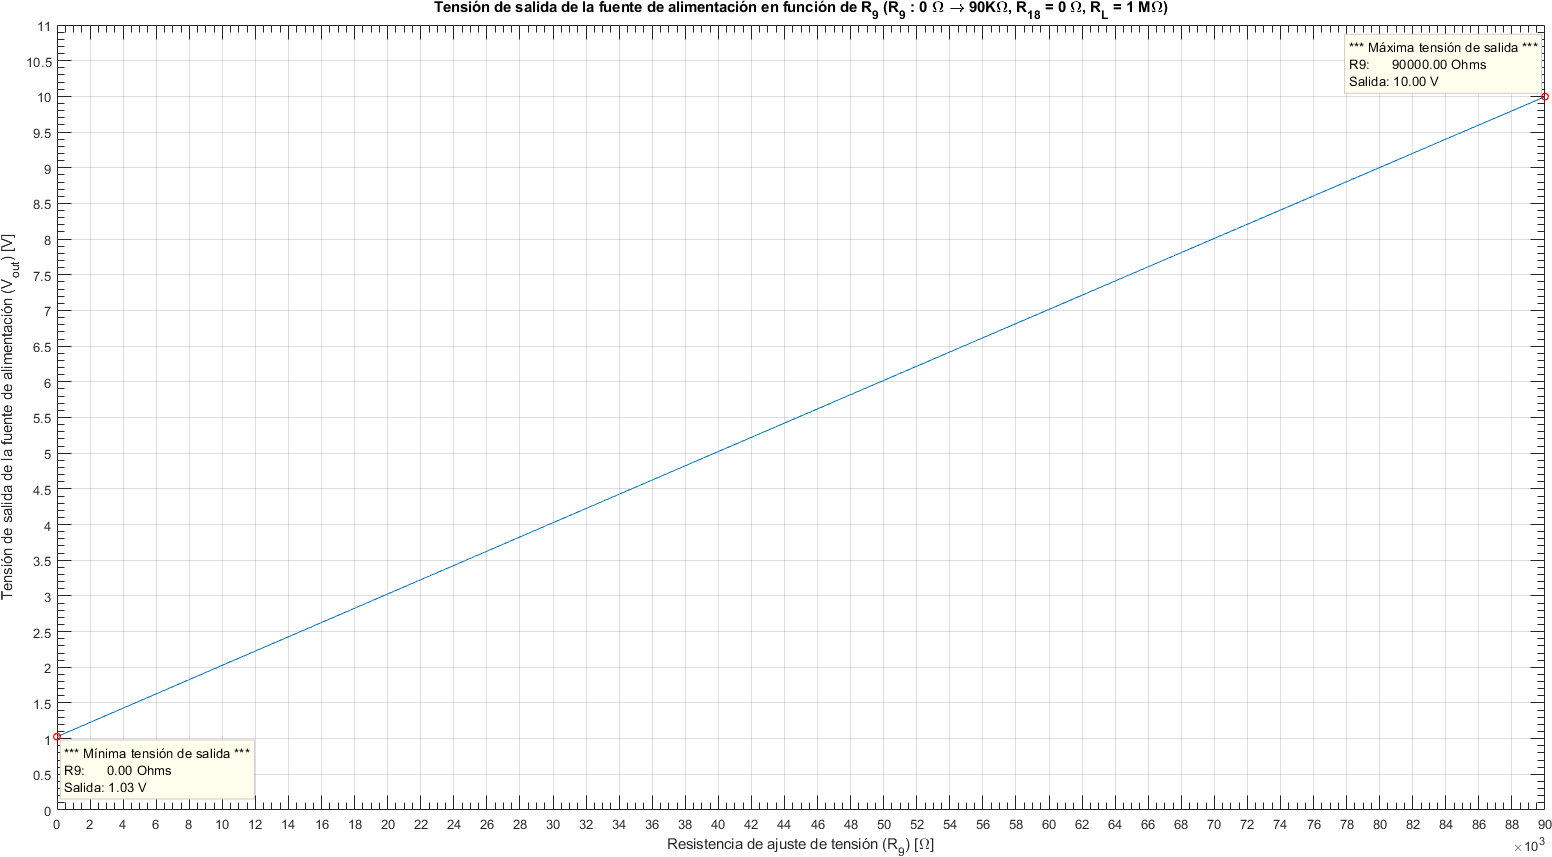
\includegraphics[width=1.2 \textwidth, angle=90]{./img/preguntas/p6.png}
\caption{\label{fig:fig_p6_output_voltage}\footnotesize{Tensión de salida, $V_{o}$, en función de $R_{9}$, con esta variando entre $0 \si[per-mode=symbol]{\ohm}$ y $90 \si[per-mode=symbol]{\kilo\ohm}$.}}
\end{center}
\end{figure}



\clearpage

\subsection{Punto 7}

\textbf{Enunciado}: 

\textsl{Calcular el factor de amortiguamiento para frecuencias medias ($1 \si[per-mode=symbol]{\kilo\hertz}$).}

\vspace{1.5cm}

El factor de amortiguamiento, $DF$ (damping factor), es la relación entre la impedancia especificada de la carga, $8 \si[per-mode=symbol]{\ohm}$ en este caso, y la impedancia de salida del amplificador, ambas consideradas como resistivas puras, a frecuencias medias, se tiene entonces:


\begin{equation}
\boxed{ DF = \frac{R_{L}}{R_{o}} = \frac{8 \si[per-mode=symbol]{\ohm}}{29.6 \si[per-mode=symbol]{\milli\ohm}} \approx 270.3 }
\end{equation}


\vfill

\clearpage



\subsection{Punto 8}

\textbf{Enunciado}: 

\textsl{Calcular la máxima tensión pico sobre la carga para frecuencias medias ($1 \si[per-mode=symbol]{\kilo\hertz}$).}

\vspace{1.5cm}

\label{punto8}

Para obtener la máxima tensión pico sobre la carga, debemos hacer la suposición que la misma se obtiene al límite donde los transistores del amplificador están al borde salir de modo activo directo, en general no son solo los transistores de la etapa de salida, sino que dependiendo la configuración el límite será impuesto por los transistores de mas de una etapa.\\

En particular para este amplificador podemos ver que para los ciclos positivo de la señal, lo siguiente:

\begin{equation} \label{eq:1}
\hat{V}_{L{max}} + V_{BE_{407}} + V_{BE_{405}} + \hat{V}_{R_{421_{max}}} = V_{CC}
\end{equation}

Condición que lleva a $Q_{407}$ y $Q_{405}$ al límite de la saturación, por supuesto en esta condición la distorsión por alinealidad será  máxima, pero mas allá el amplificador comenzará a recortar.

además tenemos que:

\begin{equation} \label{eq:2}
\hat{V}_{R_{421_{max}}} = \hat{I}_{L_{max}} \cdot R_{421} = \frac{\hat{V}_{L{max}}}{R_{L}}
\end{equation}

Combinando \ref{eq:1} y \ref{eq:2} tenemos:

\begin{equation} \label{eq:3}
\hat{V}_{L{max}} = \frac{V_{CC} - V_{BE_{407}} - V_{BE_{405}} }{1 + \frac{R_{421}}{R_{L}} }
\end{equation}


Pero \ref{eq:3} es una expresión trascendente , ya que $V_{BE_{405}}$ y $V_{BE_{407}}$ dependen de la corriente de colector de cada transistor. Asumiendo para el par una relación de $\beta$ veces en las corrientes, se tiene:


\begin{equation} \label{eq:3}
 \hat{I}_{C_{407_{max}}} = \frac{\hat{I}_{L_{max}}}{1 + \frac{1}{\beta_{407}} } = \frac{\hat{V}_{L_{max}}}{ R_{L} \cdot \left( 1 + \frac{1}{\beta_{407}} \right) }
\end{equation}

Podemos operar iterativamente usando las curvas de $I_{C} = f_{\left( V_{BE} \right)}$ de cada transistor, \textbf{Figura~10},\, \quotemarks{On~Voltages}, de la hoja de datos del transistor \textbf{TIP41}, apéndice~\sectref{datasheet_TIP41}, y \textbf{Figura~4}, \quotemarks{\mbox{Base-Emitter~On~Voltage}}, de la hoja de datos del transistor \textbf{BD135}, apéndice~\sectref{datasheet_BD135}, empezamos asumiendo que $V_{BE} = 0.7$ para ambos transistores, calculamos una tensión de pico máxima y con esta una corriente de colector máxima para el transistor $Q_{407}$ y de esta un nuevo valor para el $V_{BE}$, que nos permite calcular un nuevo valor para la tensión pico máxima, en este caso con una iteración es suficiente, se obtiene:

\begin{equation} \label{eq:3}
\boxed{\hat{V}_{L{max}} = 26.6 \si[per-mode=symbol]{\volt}}
\end{equation}

Para el ciclo negativo se obtiene un valor cercano, haciendo un análisis similar, pero que involucra a los transistores $Q_{406}$ y $Q_{404}$, tomamos este valor para el ciclo positivo, de todos modos es solo una aproximación. 



\vfill

\clearpage


\subsection{Punto 9}

\textbf{Enunciado}: 

\textsl{Calcular la máxima eficiencia obtenible con éste amplificador para frecuencias medias ($1 \si[per-mode=symbol]{\kilo\hertz}$).}

\vspace{1.5cm}

Para calcular la máxima eficiencia del amplificador, utilizamos la definición de eficiencia:

\begin{equation}
\eta_{max} = max\left\{ \frac{P_{L}}{P_{sources}} \right\} \cdot 100\%
\end{equation}

Donde $P_{L}$ es la potencia entregada a la carga y $P_{sources}$ es la potencia entregada por las fuentes de alimentación. Se puede observar fácilmente que la potencia consumida por todos los transistores que trabajan en \textbf{clase A}, no varía, salvo al tener señal aplicada, parte de esa potencia es entregada a la siguiente etapa, pero todos los transistores, excepto los de la etapa de salida, no entregan potencia a la carga, por lo que no contribuyen a la potencia útil, solo a la consumida, con esto en mente, basta ver las corrientes de reposo de todas las ramas, excepto la de los transistores de potencia, para obtener la parte fija del consumo en la fuente. Luego para ver el cuando se da el caso de mayor eficiencia, se ve fácilmente que será cuando se entregue la máxima potencia a la carga.\\


Usando la expresión general de la potencia máxima en un \textbf{clase AB}, pero con correcciones para tener en cuenta el consumo de potencia en las primeras etapas en \textbf{clase A} y la potencia disipada en las resistencias de emisor de la etapa de salida, llamando $I_{cA}$ a la corriente que circula por las ramas de las primeras etapas, y usando los valores máximos obtenidos en la sección~\sectref{max_pot}, tenemos:


\begin{equation*}
\eta_{max} = \frac{ \frac{ \hat{I}_{L{max}} \cdot \hat{V}_{L{max}} }{2}   }{  \frac{ 2 \cdot \hat{I}_{L{max}} \cdot V_{CC}  }{ \pi } + \left( V_{CC} + V_{SS} \right) \cdot I_{cA} + \hat{I}_{L{max}} \cdot R_{421}  } \cdot 100\%
\end{equation*}\\


\begin{equation}
\boxed{ \eta_{max} = \frac{ \frac{ 3.33 \si[per-mode=symbol]{\ampere}  \cdot 26.6 \si[per-mode=symbol]{\volt} }{2}   }{  \frac{ 2 \cdot  3.33 \si[per-mode=symbol]{\ampere} \cdot 30 \si[per-mode=symbol]{\volt}  }{ \pi } + 60 \si[per-mode=symbol]{\volt} \cdot 9.25 \si[per-mode=symbol]{\milli\ampere} + 3.33 \si[per-mode=symbol]{\ampere} \cdot 0.47 \si[per-mode=symbol]{\ohm}  } \cdot 100\% \approx 67.4 \% }
\end{equation}




\vfill

\clearpage


\subsection{Punto 10}
\label{thermal}

\textbf{Enunciado}: 

\noindent{
\textsl{Determinar:}

\begin{enumerate}
\item[\textit{a)}] \textit{El tamaño de los disipadores para cada transistor (resistencia térmica disipador-ambiente).}
\item[\textit{b)}] \textit{Encontrar el disipador comercial que podría utilizarse para construir un prototipo funcional.}
\item[\textit{c)}] \textit{Comparar con los disipadores utilizados originalmente por Turner y obtener conclusiones.}
\end{enumerate}

}

\vspace{1.5cm}

\subsubsection{Tamaño de los disipadores para cada transistor (resistencia térmica disipador-ambiente)}
\label{thermal_calculation}

Primero determinamos de los puntos de trabajo calculados en la sección~\sectref{qpoint}, las potencias disipadas en cada uno de los transistores de señal y potencia media, los resultados se resumen en el cuadro~\tableref{table:table_powers}


%% \noindent
%% \begin{center}
 
%%\begin{spacing}{1}  
\begin{table}[H]  %%\centering
    
    \setlength\arrayrulewidth{1.5pt}
    \arrayrulecolor{white}
    \def\clinecolor{\hhline{|>{\arrayrulecolor{white}}-%
    >{\arrayrulecolor{white}}|-|-|-|-|-|}}
\resizebox{0.8 \textwidth}{!}{% 
       
\begin{tabularx}{1 \textwidth}%
    {|
    >{\columncolor{white} \centering\arraybackslash}m{0.29\linewidth}
     |
    >{\columncolor{white} \centering\arraybackslash}m{0.14\linewidth}
     |
    >{\columncolor{white} \centering\arraybackslash}m{0.14\linewidth}
     |
    >{\columncolor{white} \centering\arraybackslash}m{0.14\linewidth}
     |
    >{\columncolor{white} \centering\arraybackslash}m{0.14\linewidth}
     |
    >{\columncolor{white} \centering\arraybackslash}m{0.14\linewidth}
     |
    }
    \rowcolor{HeadersColor} \cellcolor{white} \thead{}  & \thead{$Q_{402}$} & \thead{$Q_{403}$} & \thead{$Q_{404}$} & \thead{$Q_{405}$} & \thead{$Q_{406}$} \\
    
    \hhline{|-|-|-|-|-|}
    \rowcolor{gray!20} \cellcolor{gray!40} $I_{C}$ [$\si[per-mode=symbol]{\milli\ampere}$] & $0.54$ & $8.66$ & $9$ & $6$ & $5.5$  \\
    \hhline{|-|-|-|-|-|}
    \rowcolor{gray!20} \cellcolor{gray!40} $V_{CE}$ [$\si[per-mode=symbol]{\volt}$] & $26.1$ & $1.8$ & $27.95$ & $29.4$ & $29.4$  \\
    \hhline{|-|-|-|-|-|}
    \rowcolor{Butter!20} \cellcolor{gray!40}  $P_{D}$ [$\si[per-mode=symbol]{\watt}$] & $14.1 \si[per-mode=symbol]{\milli}$ & $15.6 \si[per-mode=symbol]{\milli}$ & $251 \si[per-mode=symbol]{\milli}$ & $228 \si[per-mode=symbol]{\milli}$ & $228 \si[per-mode=symbol]{\milli}$ \\
    \hhline{|-|-|-|-|-|}
    \rowcolor{gray!20} \cellcolor{gray!40} \thead{\cellcolor{gray!40} \color{black} $P_{D_{max}}^{*}$ [$\si[per-mode=symbol]{\watt}$] } & $625 \si[per-mode=symbol]{\milli}$ & $625 \si[per-mode=symbol]{\milli}$ & $1.25$ & $1.25$ & $1.25$  \\
    \hhline{|-|-|-|-|-|}  
    \rowcolor{gray!20} \cellcolor{gray!40} \thead{\cellcolor{gray!40} \color{black} $\theta_{ja}^{*}$ [$\si[per-mode=symbol]{\celsius\per\watt}$] } & $200$ & $200$ & $100$ & $100$ & $100$  \\
    \hhline{|-|-|-|-|-|}  
    \rowcolor{gray!20} \cellcolor{gray!40} \thead{\cellcolor{gray!40} \color{black} $\theta_{jc}^{*}$ [$\si[per-mode=symbol]{\celsius\per\watt}$] } & $83.3$ & $83.3$ & $10$ & $10$ & $10$  \\
    \hhline{|-|-|-|-|-|}     
       
    \end{tabularx}}
	\caption{\footnotesize{Potencia disipada en los transistores de señal y media potencia.}}
	\label{table:table_powers}
\end{table}
%%\end{spacing}

%% \end{center}

\footnotesize{
$\left(*\right)$ Los datos se tomaron de las correspondientes hojas de datos.
}\\\\


Para todos los transistores que trabajan en \textbf{clase A}, $Q_{402}$, $Q_{403}$ y $Q_{404}$, las potencias disipadas se calcularon simplemente como $V_{CE} \cdot I_{C}$, ya que esto corresponde a la máxima potencia disipada en el transistor, que se da cuando no hay señal en el mismo.\\

Para los transistores $Q_{405}$ y $Q_{406}$, los drivers de los pares compuestos que integran la etapa de salida en \textbf{clase AB}, se hizo las siguientes  suposiciones simplificadoras, que la tensión \mbox{colector-emisor} en los mismos coincide con la de los transistores de salida y que por los mismos circula una corriente que es $\beta$ veces menor que en los transistores de salida, de esta forma la potencia termina siendo $\beta$ veces menor que en estos. De todas formas se trata de unas suposiciones conservadoras.\\

Para los dos transistores de salida, la potencia máxima disipada se calcula como:

\begin{equation}
      P_{C_{max_{Q_{407}}}} = P_{C_{max_{Q_{4088}}}} = \frac{{V_{CC}}^2}{{\pi}^2 \cdot R_{L}} = 11.4 \si[per-mode=symbol]{\watt}
\end{equation}\\

Y se obtiene entonces para los transistores drivers de los pares:

\begin{equation}
P_{C_{max_{Q_{405}}}} = P_{C_{max_{Q_{406}}}} = \frac{P_{C_{max_{Q_{7}}}}}{\beta_{407}} = \frac{11.4 \si[per-mode=symbol]{\watt}}{50} = 228 \si[per-mode=symbol]{\milli\watt}
\end{equation}\\

Para determinar la necesidad de un disipador térmico en cada uno de los transistores, suponemos su operación sin el mismo y planteamos el circuito térmico correspondiente. Para este planteo se necesitan también los siguientes parámetros:

\begin{enumerate}
\item[$\bm{T_{j_{max}}}$] Temperatura máxima de operación de la juntura del transistor ($150 \si[per-mode=symbol]{\celsius}$ para todos los transistores analizados).
\item[$\bm{T_{j_{e}}}$] Temperatura de operación estimada de la juntura del transistor.
\item[$\bm{T_{a}}$] Temperatura ambiente (tomamos $40 \si[per-mode=symbol]{\celsius}$ como un caso de un circuito encerrado en un gabinete).
\item[$\bm{\theta_{ja}}$] Resistencia térmica de la juntura del transistor al ambiente.\\
\end{enumerate}


Entonces solo tenemos una fuente de potencia, $P_{D}$ (modelada por una fuente de corriente) circulando por la resistencia térmica $\theta_{ja}$ (modelada como una resistencia eléctrica), con lo que la temperatura (modelada por tensión) que se desarrolla sobre la juntura se suma a la temperatura ambiente (modelada por una fuente de tensión), con lo que nos queda:


\begin{equation} \label{eq:thermal_ambient}
T_{j_{e}} = P_{D} \cdot \theta_{ja} + T_{a}
\end{equation}\\

Nos queda para cada uno de los transistores de señal y para los drivers de los pares:

\begin{enumerate}
\item[$\bm{Q_{402}}$] $T_{j_{e_{402}}} = 41.2 \si[per-mode=symbol]{\celsius} $ 
\item[$\bm{Q_{403}}$] $T_{j_{e_{403}}} = 41.3 \si[per-mode=symbol]{\celsius} $ 
\item[$\bm{Q_{404}}$] $T_{j_{e_{404}}} = 65.1 \si[per-mode=symbol]{\celsius} $
\item[$\bm{Q_{405}}$] $T_{j_{e_{405}}} = 62.8 \si[per-mode=symbol]{\celsius} $
\item[$\bm{Q_{406}}$] $T_{j_{e_{406}}} = 62.8 \si[per-mode=symbol]{\celsius} $
\item[$\bm{Q_{407}}$] $T_{j_{e_{407}}} = 62.8 \si[per-mode=symbol]{\celsius} $
\item[$\bm{Q_{408}}$] $T_{j_{e_{408}}} = 62.8 \si[per-mode=symbol]{\celsius} $
\end{enumerate}

Podemos ver que ninguno de los transistores supera la máxima temperatura de trabajo, con lo que concluimos que no necesitan disipador térmico.\\

Para los transistores de salida, ambos son el mismo tipo de transistor, obtenemos las resistencias térmicas de la \textbf{figura 7}, \quotemarks{Power Derating} de la hoja de datos del transistor \textbf{TIP41}, apéndice~\sectref{datasheet_TIP41}. Obtenemos:\\

$\theta_{ja_{Q_{407}}} = \theta_{ja_{Q_{408}}} = 60 \si[per-mode=symbol]{\celsius\per\watt}$ y $\bm{\theta_{jc_{Q_{407}}}} = \bm{\theta_{jc_{Q_{408}}}} = 1.9 \si[per-mode=symbol]{\celsius\per\watt} $.\\

Si aplicamos la expresión~\ref{eq:thermal_ambient} nuevamente, obtenemos para ambos transistores de salida:\\

$T_{j_{e_{407}}} = T_{j_{e_{408}}} =  724 \si[per-mode=symbol]{\celsius} $\\

Muy por encima de la temperatura máxima de trabajo para la juntura, con lo que es necesario un disipador térmico. Para calcular la resistencia térmica máxima del disipador que se necesita, se plantea un circuito térmico, pero ahora conteniendo las resistencias térmicas de la juntura al encapsulado, del encapsulado al disipador y del disipador al ambiente, esta última es la que se necesita determinar, en la figura~\figref{fig:fig_thermal_circuit} se muestra el circuito térmico completo.


\begin{figure}[H] %htb
\begin{center}
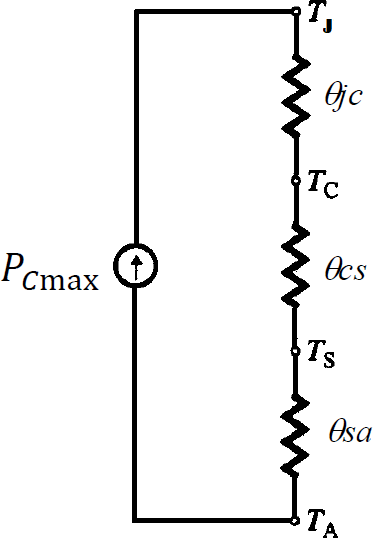
\includegraphics[width=0.35 \textwidth, angle=0]{./img/desarrollo/thermal_circuit.png}
\caption{\label{fig:fig_thermal_circuit}\footnotesize{Circuito térmico para los transistores de salida.}}
\end{center}
\end{figure}

Del planteo de este circuito se despeja la expresión para la resistencia térmica del disipador, $\theta_{sa}$, se obtiene:

\begin{equation}
\theta_{sa} = \frac{T_{J} - T_{a}}{P_{C_{max}}} - \theta_{jc} - \theta_{cs}
\end{equation}


Donde $\theta_{jc}$ ya se obtuvo de las hojas de datos y $\theta_{cs}$, la resistencia térmica del encapsulado al disipador, depende del montaje mecánico que se realiza del transistor sobre el disipador, el mismo puede ser con mica, grasa siliconada, o ambas, el transistor se puede justar mas o menos sobre la superficie del disipador, etc. Teniendo en cuenta estas variantes se estima que $1 \si[per-mode=symbol]{\celsius\per\watt} \leq \theta_{cs} \geq 0.5 \si[per-mode=symbol]{\celsius\per\watt} $, tomamos $1 \si[per-mode=symbol]{\celsius\per\watt}$, el peor caso. Obtenemos entonces para los transistores de salida:

\begin{equation}
\theta_{sa_{max}} = \frac{T_{J} - T_{a}}{P_{C_{max}}} - \theta_{jc} - \theta_{cs} = \frac{150 \si[per-mode=symbol]{\celsius} - 40 \si[per-mode=symbol]{\celsius}   }{11.4  \si[per-mode=symbol]{\watt} } - 1.9 \si[per-mode=symbol]{\celsius\per\watt} - 1 \si[per-mode=symbol]{\celsius\per\watt} \approx 6.8 \si[per-mode=symbol]{\celsius\per\watt}\\ \\
\end{equation}

Con lo que solo necesitamos disipadores para los transistores de salida que cumplan:

\begin{center}
\begin{equation}
\boxed{ \theta_{sa} \leq 6.8 \si[per-mode=symbol]{\celsius\per\watt} }
\end{equation}
\end{center}

\clearpage

\subsubsection{Disipador comercial que podría utilizarse para construir un prototipo funcional}

En la sección anterior calculamos la resistencia térmica que debe tener el disipador térmico de los transistores de salida, se encontró que, $\theta_{sa} \leq 6.8 \si[per-mode=symbol]{\celsius\per\watt}$, usando este valor como referencia se seleccionó un disipador que sería adecuado, el mismo se muestra en la figura~\figref{fig:fig_thermal_dissipator}, tiene $\theta_{sa} = 5.1 \si[per-mode=symbol]{\celsius\per\watt}$, es el modelo \textbf{6225M ZD-5}.

\begin{figure}[H] %htb
\begin{center}
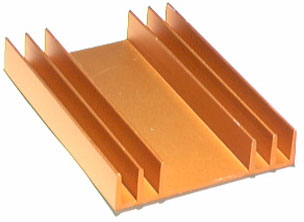
\includegraphics[width=0.6 \textwidth, angle=0]{./img/desarrollo/10b_6225M_ZD_5.png}
\caption{\label{fig:fig_thermal_dissipator}\footnotesize{Disipador térmico seleccionado (\textbf{6225M ZD-5}).}}
\end{center}
\end{figure}


\subsubsection{Comparación con los disipadores utilizados originalmente por Turner}

No pudimos encontrar información acerca del valor de la resistencia térmica de los disipadores usados originalmente, pero de las fotos que hay disponibles, los disipadores eran tipo \textbf{U}, el tamaño y el largo aparente de las aletas hacen parecer que tiene una masa metálica aproximadamente del mismo tamaño, pero no hay mucho mas que podamos decir, salvo que es probable que los disipadores hayan sido sobre-dimensionados al tratarse de un producto comercial, y que probablemente la temperatura interna del gabinete sea superior a la que nosotros consideramos.




\clearpage



\subsection{Punto 11}
\label{simulations}
\textbf{Enunciado}: 

\noindent{
\textsl{Simular el comportamiento estático y dinámico del amplificador determinando:}

\begin{enumerate}
\item[\textit{a)}] \textit{Medir las tensiones de todos los nodos y las corrientes de todas la ramas para $V_{G} = 0 \si[per-mode=symbol]{\volt}$.}
\item[\textit{b)}] \textit{Medir la impedancia de entrada en función de la frecuencia (desde $0.1 \si[per-mode=symbol]{\hertz}$ hasta $1 \si[per-mode=symbol]{\giga\hertz}$).}
\item[\textit{c)}] \textit{Medir la impedancia de salida en función de la frecuencia (desde $0.1 \si[per-mode=symbol]{\hertz}$ hasta $1 \si[per-mode=symbol]{\giga\hertz}$).}
\item[\textit{d)}] \textit{Respuesta en frecuencia para $1 \si[per-mode=symbol]{\watt}$ sobre la carga.}
\item[\textit{e)}] \textit{Ancho de banda de potencia.}

\textit{Es la máxima frecuencia para la que el amplificador logra reproducir una señal sinusoidal a máxima potencia (hallada en el punto 4) sin deformación.}

\item[\textit{f)}] \textit{Respuesta al escalón}

\begin{enumerate}
\item[\textit{i.}] \textit{Pequeña señal (la tensión pico de salida estará entre $0.1 \si[per-mode=symbol]{\volt}$ y $1 \si[per-mode=symbol]{\volt}$).}
\item[\textit{ii.}] \textit{Gran señal (amplitud de salida apenas menor que la máxima tensión pico de salida hallada en el punto 8.}
\item[\textit{iii.}] \textit{En base a lo medido en i. determinar el ancho de banda para pequeña señal asumiendo que el amplificador está compensado por polo dominante.}
\item[\textit{iv.}] \textit{En base a lo medido en ii. determinar la velocidad de crecimiento de la tensión de salida (\mbox{\quotemarks{slew rate}}).}
\end{enumerate}

\item[\textit{g)}] \textit{Determinar el margen de fase.}
\item[\textit{h)}] \textit{Determinar la distorsión armónica a $1 \si[per-mode=symbol]{\kilo\hertz}$ y a $10 \si[per-mode=symbol]{\kilo\hertz}$ para potencias de $0.1 \si[per-mode=symbol]{\watt}$, $1 \si[per-mode=symbol]{\watt}$, $10 \si[per-mode=symbol]{\watt}$ y $90\%$ de la máxima calculada en el punto 4.}
\item[\textit{i)}] \textit{Determinar la distorsión por intermodulación para potencias de $0.1 \si[per-mode=symbol]{\watt}$, $1 \si[per-mode=symbol]{\watt}$, $10 \si[per-mode=symbol]{\watt}$ y $90\%$ de la máxima calculada en el punto 4.}
\item[\textit{j)}] \textit{Determinar el Rechazo de Ruido de la Fuente de Alimentación (\mbox{\quotemarks{PSNR}}).}
\end{enumerate}
}


\vspace{1.5cm}

\clearpage

\subsubsection{Punto de reposo hallado por simulación}

En la figura~\figref{fig:fig_simulated_qpoint} se muestra lo hallado por simulación para el circuito. Vemos una gran similitud con los valores calculados anteriormente, figura~\figref{fig:fig_calculated_qpoint}, aunque hubo que cambiar el valor de $PS_{401}$ con respecto al calculado para acercarnos lo más posible a $0 \si[per-mode=symbol]{\volt}$ en la salida, y también se tuvo que cambiar el valor de $PS_{402_{A}}$ y $PS_{402_{B}}$ para asegurar $10 \si[per-mode=symbol]{\milli\ampere}$ en los colectores de $Q_{407}$ y $Q_{408}$.


\begin{figure}[H] %htb
\begin{center}
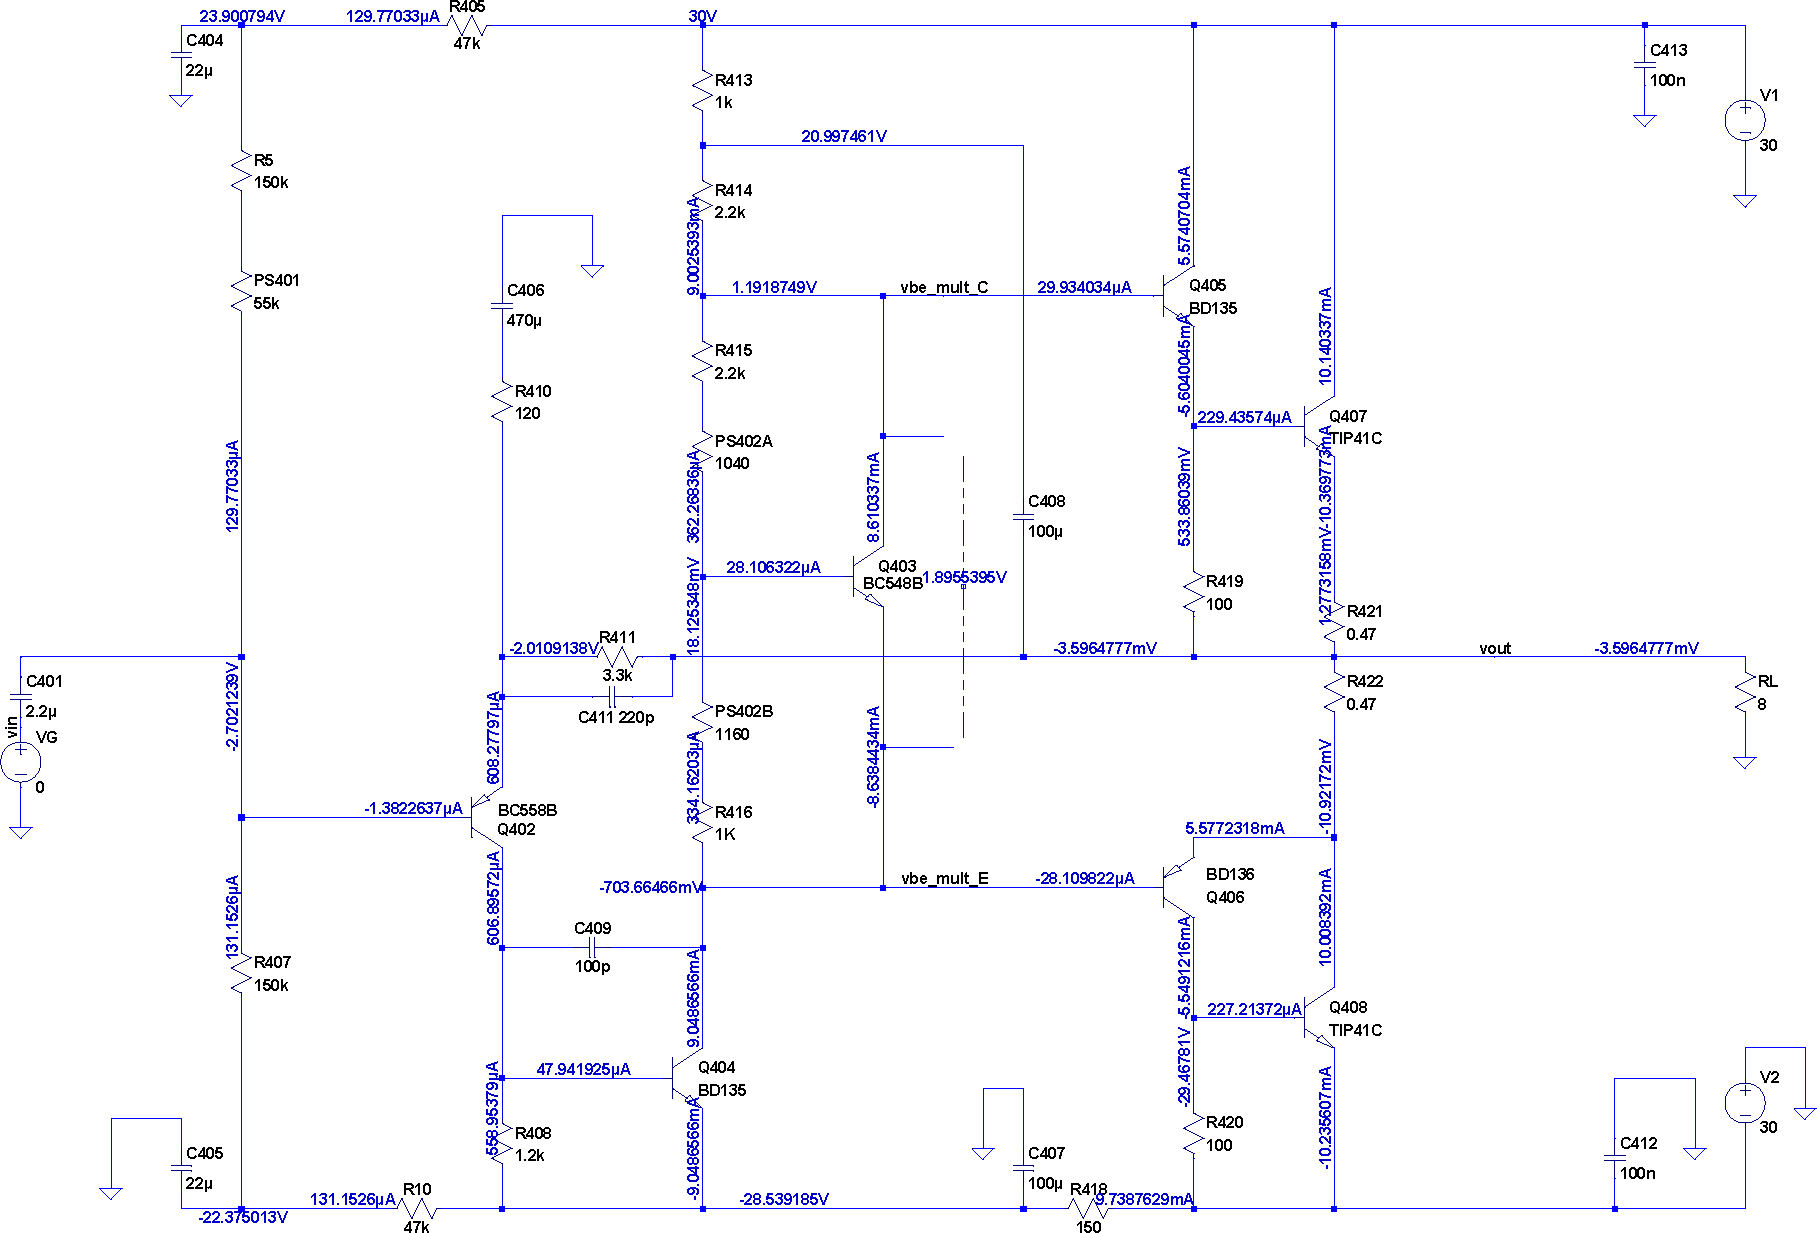
\includegraphics[width=0.9 \textwidth, angle=90]{./img/circuitos_usados/P1_P11a_qpoint.png}
\caption{\label{fig:fig_simulated_qpoint}\footnotesize{Punto de reposo del circuito hallado por simulación.}}
\end{center}
\end{figure}


\clearpage

\subsubsection{Impedancia de entrada hallada por simulación}

En la figura~\figref{fig:fig_simulated_zi} se muestra lo obtenido al simular para obtener la impedancia de entrada, el valor a frecuencias medias $86.02 \si[per-mode=symbol]{\kilo\ohm}$ se acerca bastante al valor calculado en la sección~\sectref{calculated_zi}, se había calculado $85.3 \si[per-mode=symbol]{\kilo\ohm}$.


\begin{figure}[H] %htb
\begin{center}
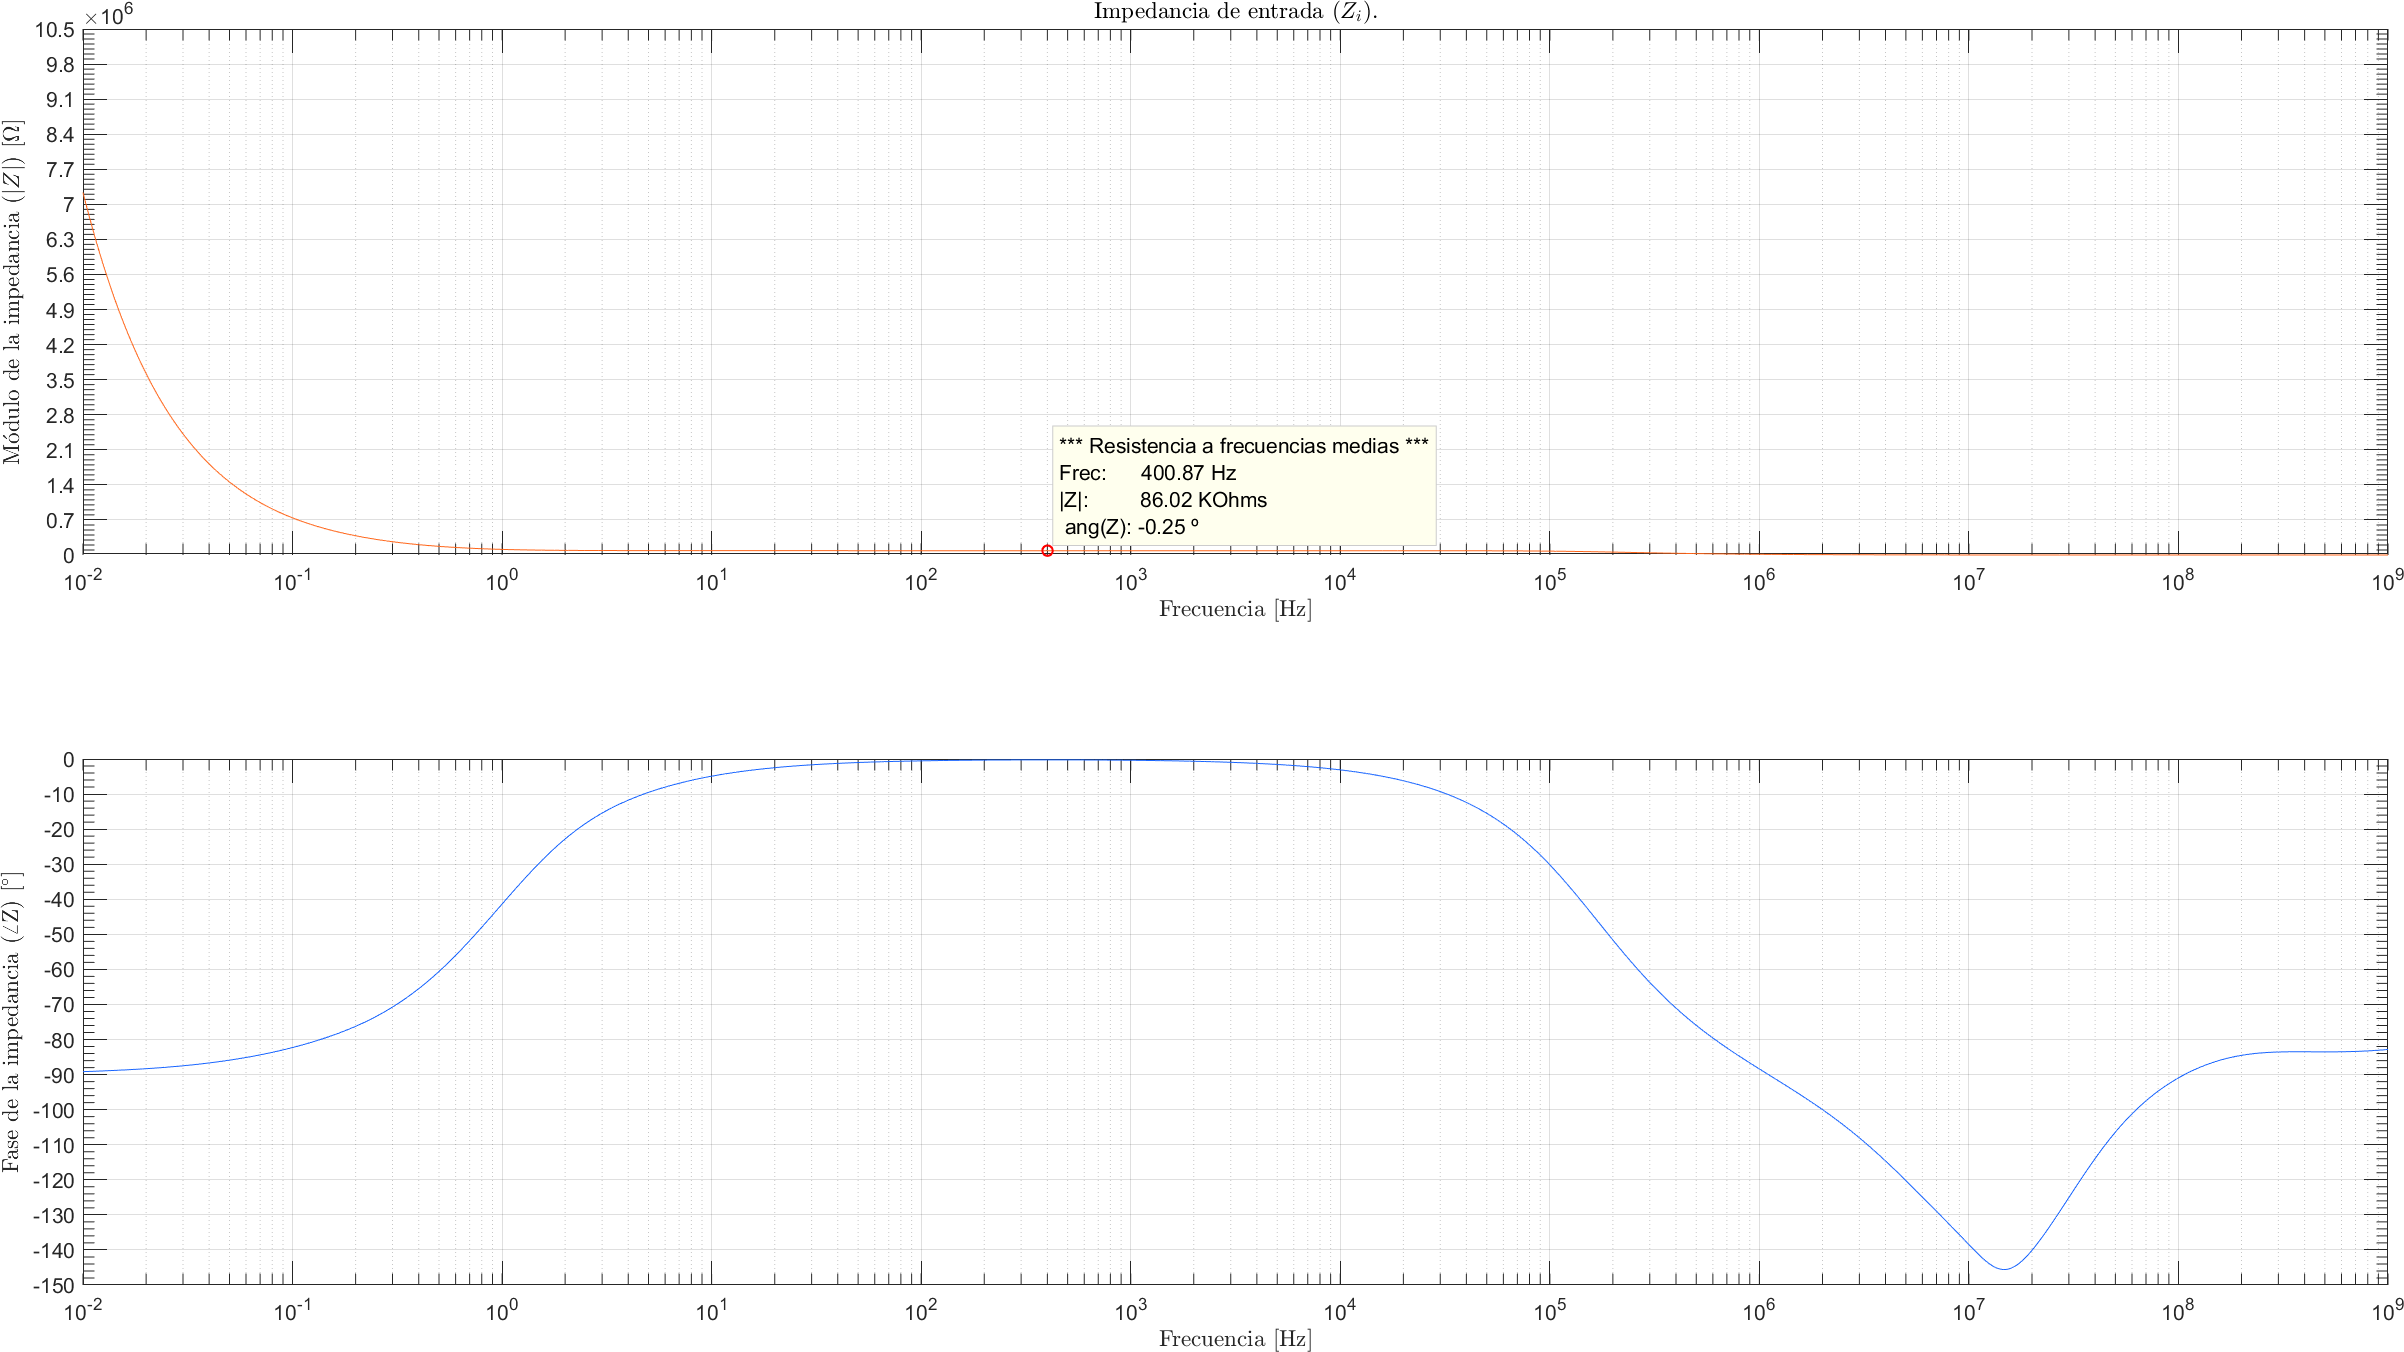
\includegraphics[width=0.9 \textwidth, angle=90]{./img/puntos/P11b_Ri.png}
\caption{\label{fig:fig_simulated_zi}\footnotesize{Impedancia de entrada hallada por simulación.}}
\end{center}
\end{figure}



\clearpage

\subsubsection{Impedancia de salida hallada por simulación}

En la figura~\figref{fig:fig_simulated_zo} se muestra lo obtenido al simular para obtener la impedancia de salida, el valor a frecuencias medias $17.58 \si[per-mode=symbol]{\milli\ohm}$ se aparta un poco del valor calculado en la sección~\sectref{calculated_zo}, se había calculado $29.6 \si[per-mode=symbol]{\milli\ohm}$, pero por lo dicho en dicha sección acerca del cálculo de la impedancia de salida a lazo abierto y por la fuerte dependencia del valor con la ganancia de lazo, que se calcula en forma aproximada, era esperable la diferencia.


\begin{figure}[H] %htb
\begin{center}
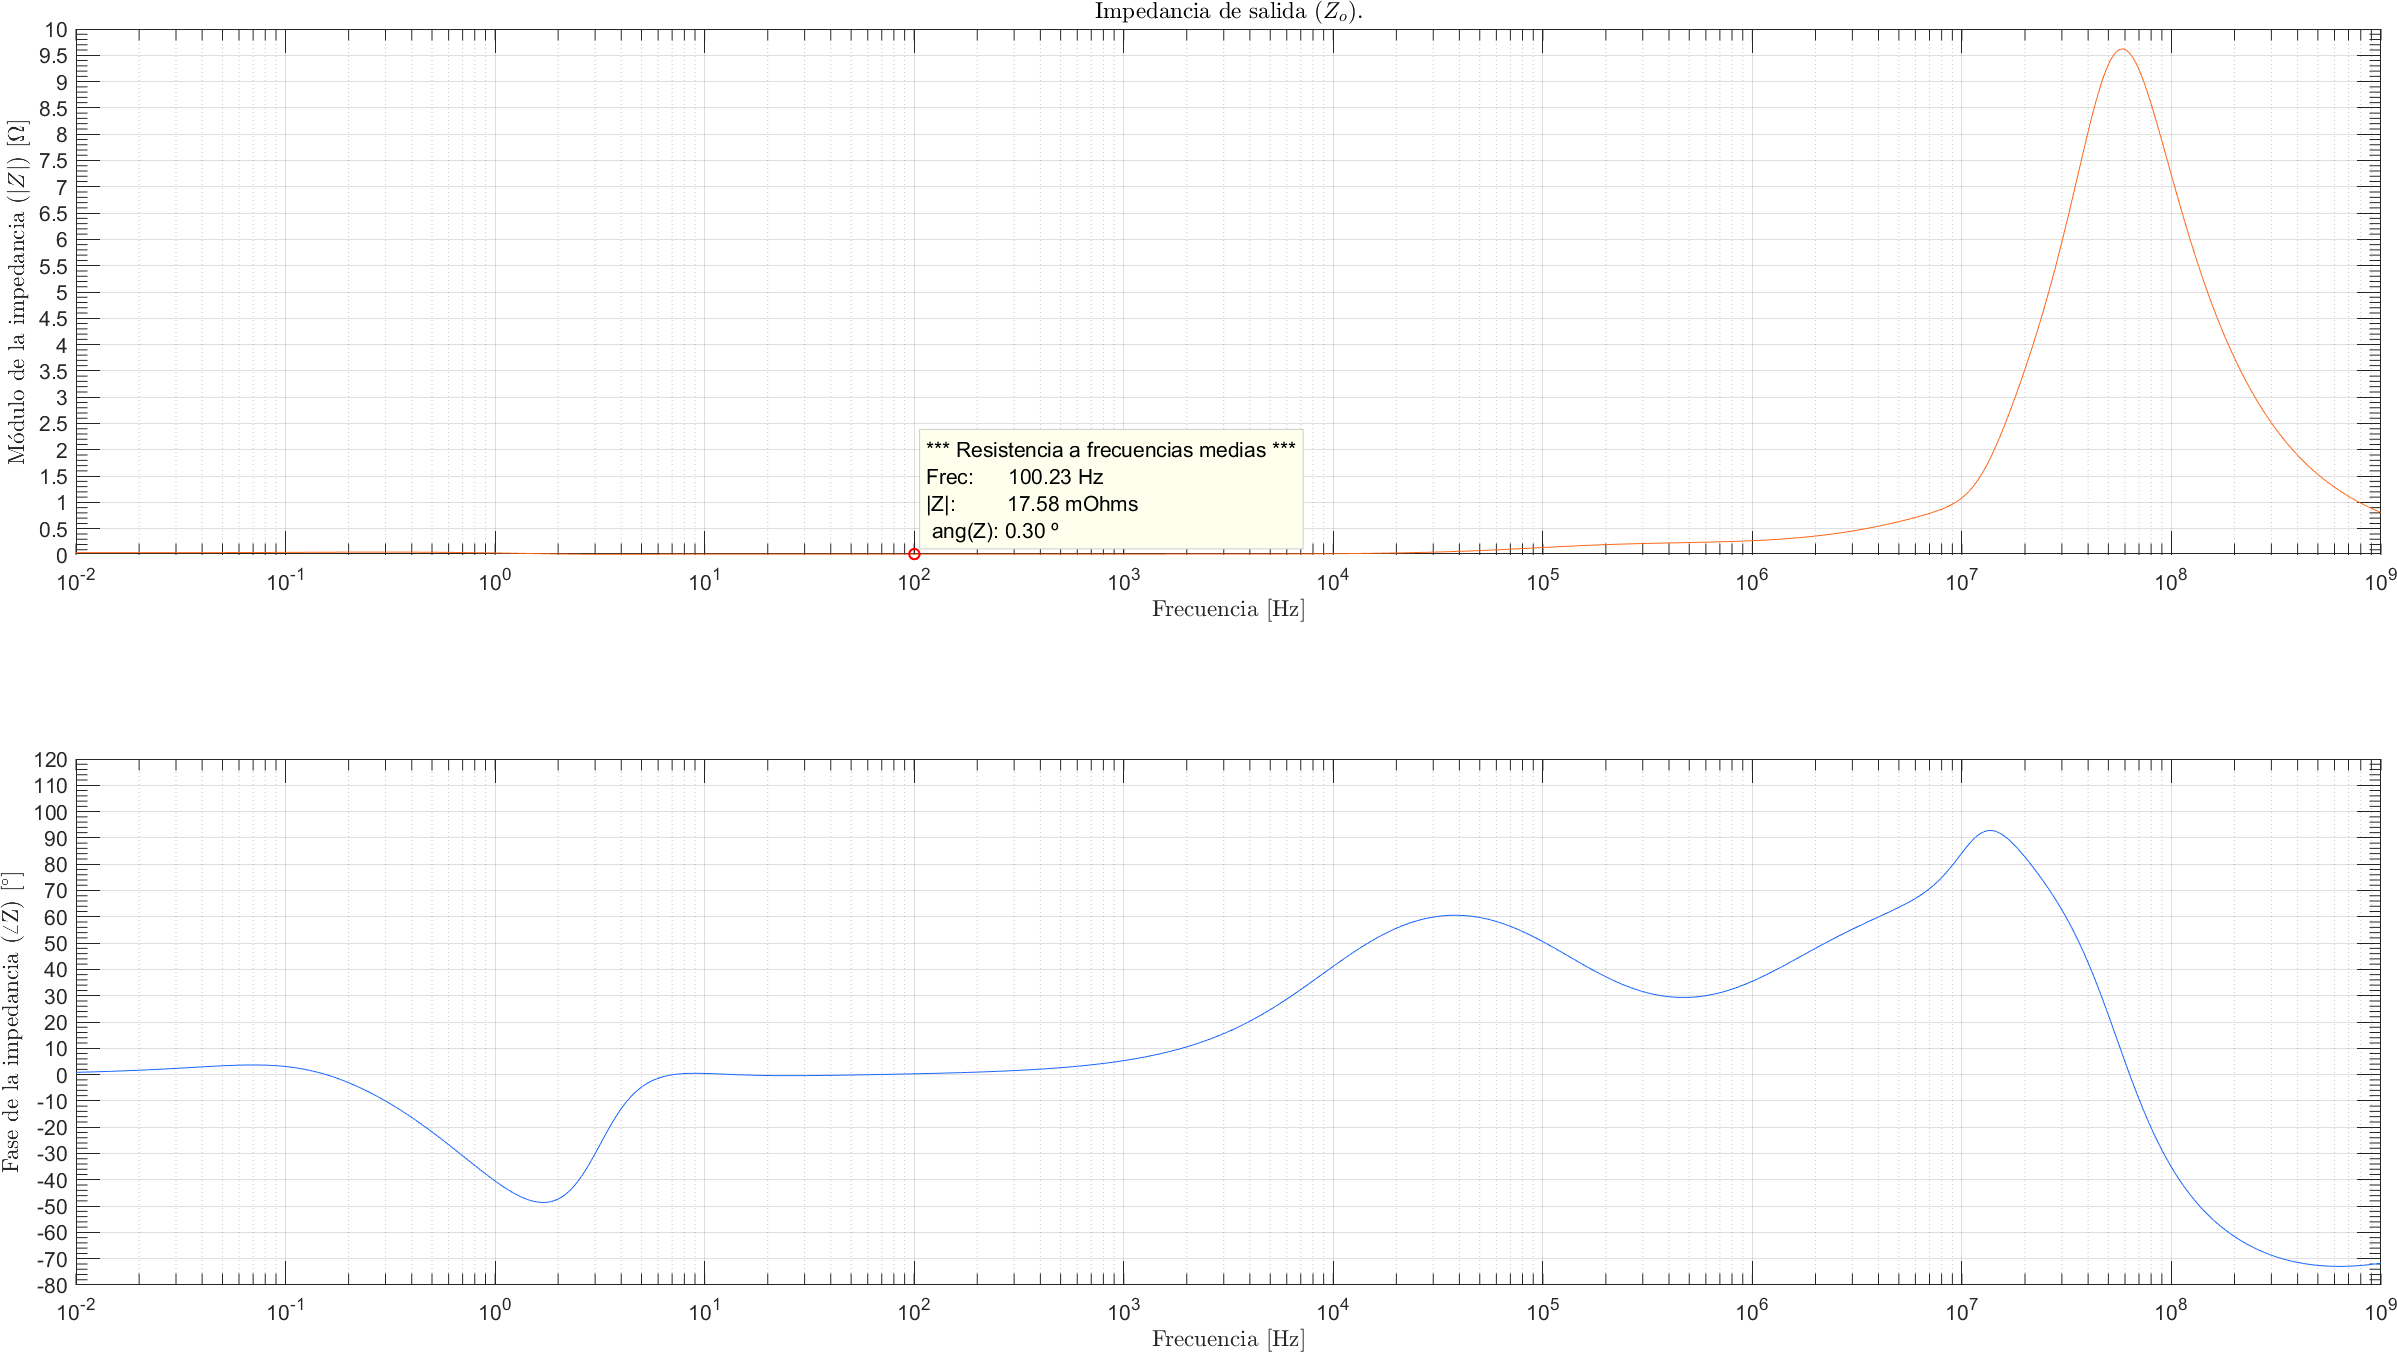
\includegraphics[width=0.9 \textwidth, angle=90]{./img/puntos/P11c_Ro.png}
\caption{\label{fig:fig_simulated_zo}\footnotesize{Impedancia de salida hallada por simulación.}}
\end{center}
\end{figure}



\clearpage

\subsubsection{Respuesta en frecuencia para $1 \si[per-mode=symbol]{\watt}$ sobre la carga}

En la figura~\figref{fig:fig_RF_1W} se muestra lo obtenido al simular para obtener la respuesta en frecuencia a $1 \si[per-mode=symbol]{\watt}$ de potencia sobre la carga, en la misma se puede ver el valor del ancho de banda encontrado, $129.55 \si[per-mode=symbol]{\kilo\hertz}$.

\begin{figure}[H] %htb
\begin{center}
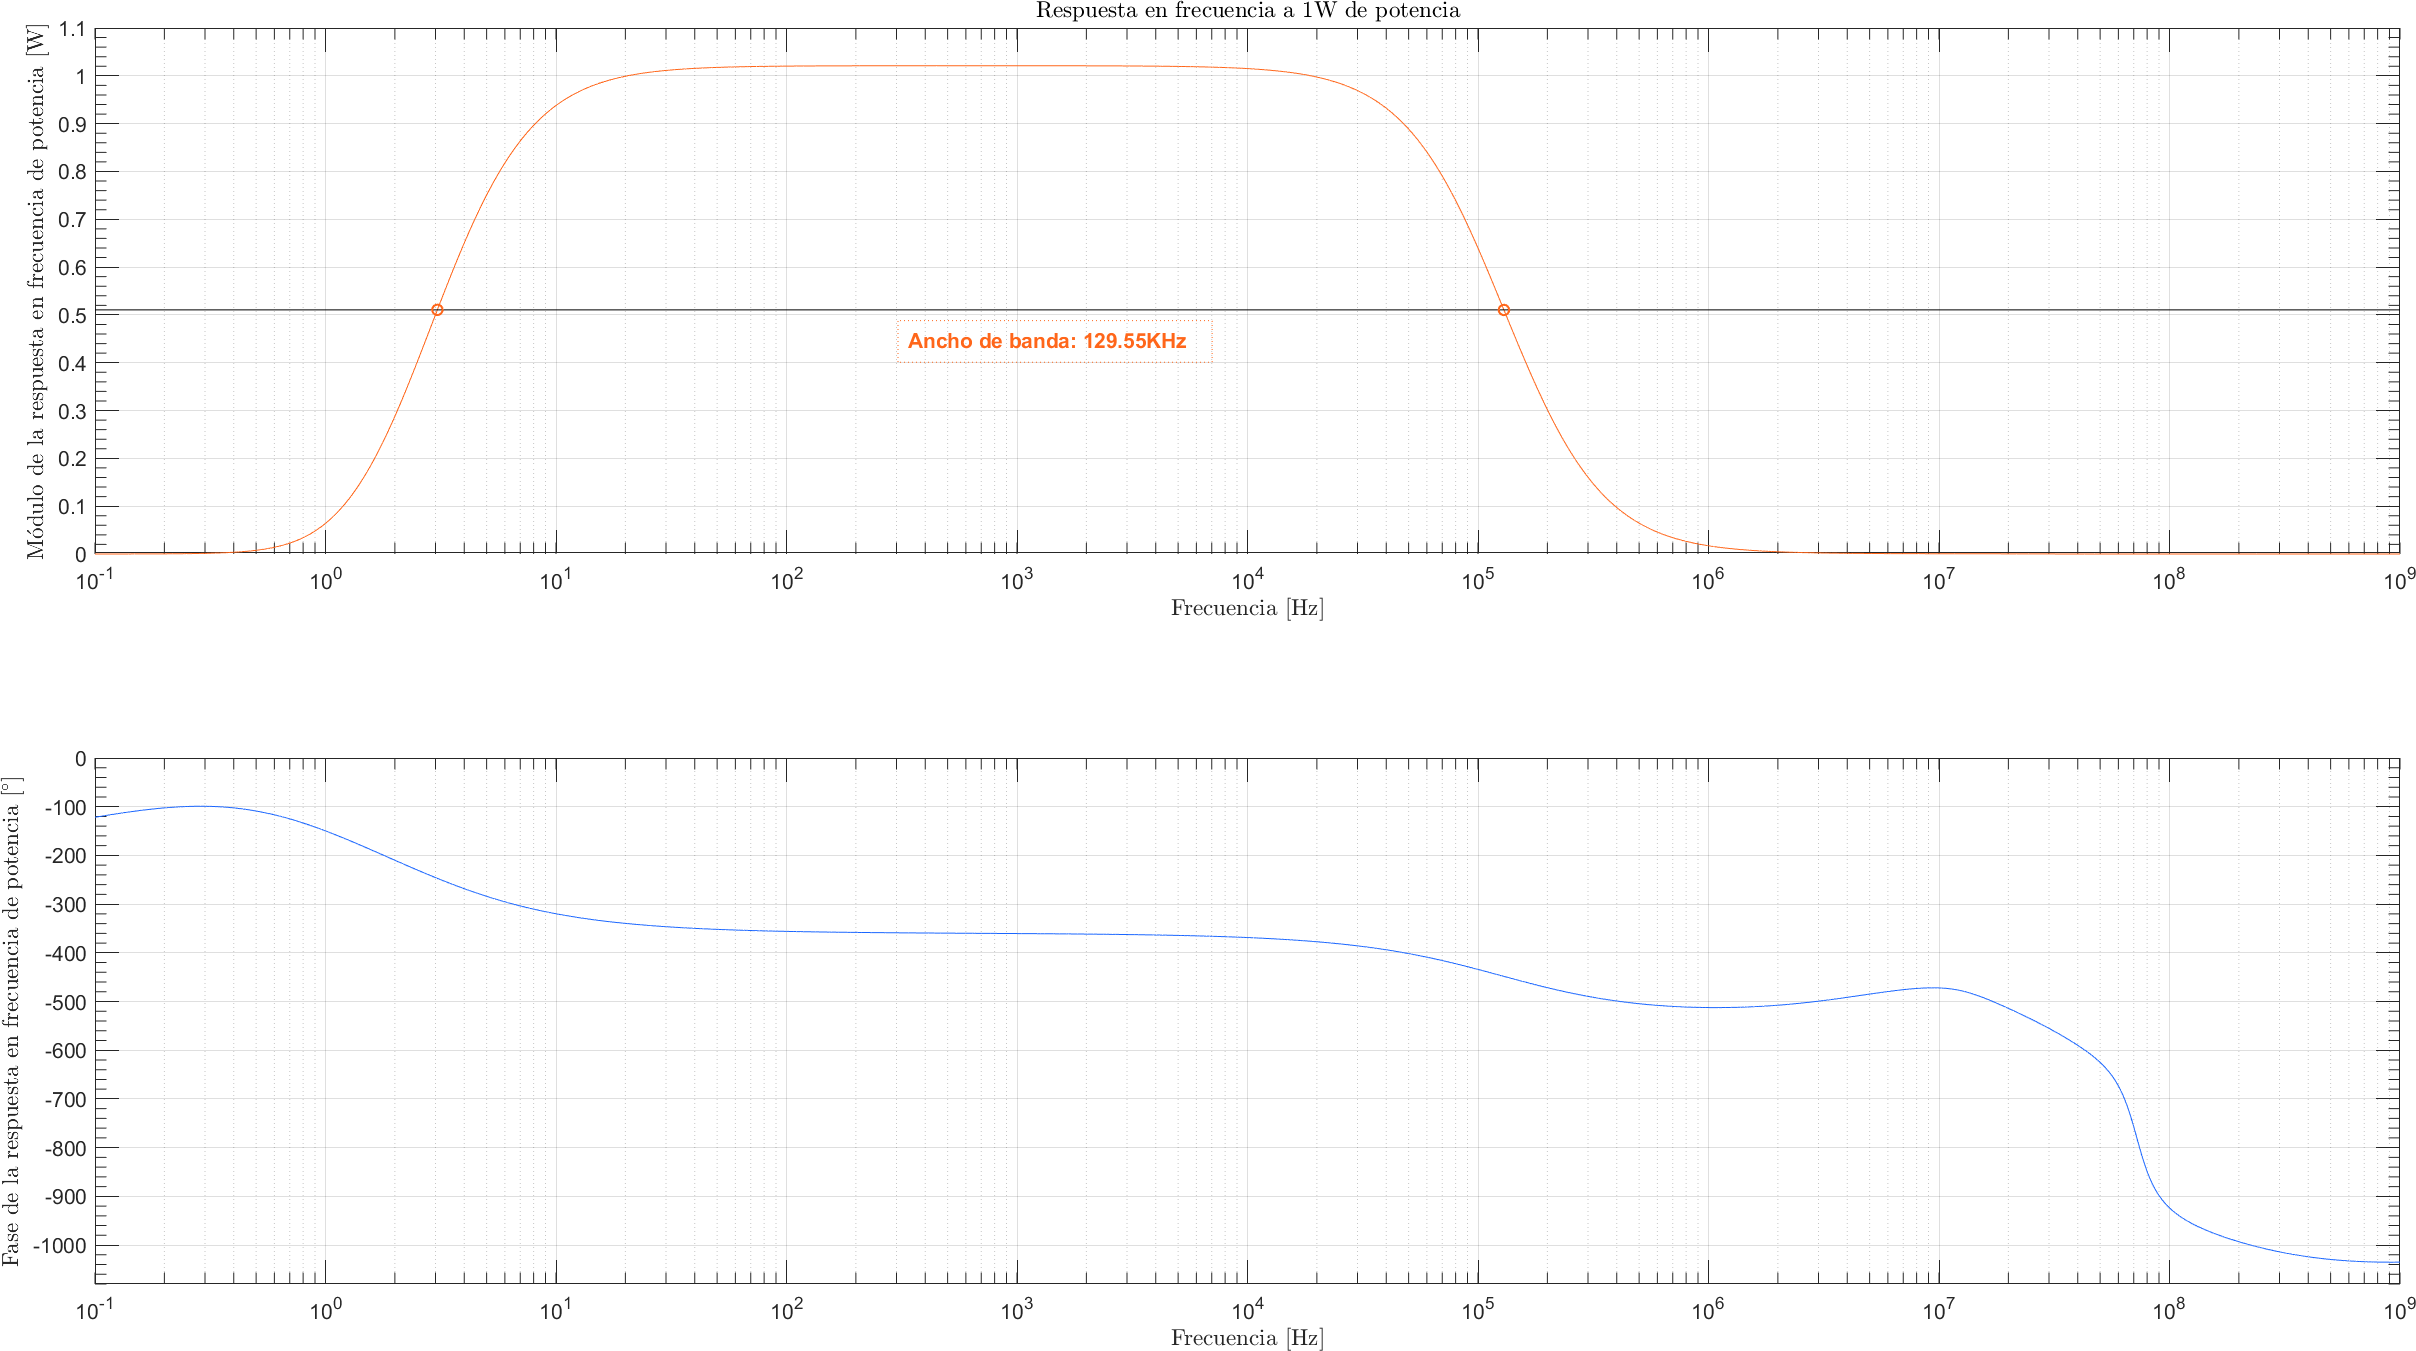
\includegraphics[width=0.9 \textwidth, angle=90]{./img/puntos/P11d_RF_1W.png}
\caption{\label{fig:fig_RF_1W}\footnotesize{Respuesta en frecuencia para $1 \si[per-mode=symbol]{\watt}$ sobre la carga.}}
\end{center}
\end{figure}


\clearpage

\subsubsection{Ancho de banda de potencia, a máxima potencia sobre la carga}

En la figura~\figref{fig:fig_RF_MAX_POWER} se muestra lo obtenido al simular para obtener la respuesta en frecuencia a $1 \si[per-mode=symbol]{\watt}$ de potencia sobre la carga, en la misma se puede ver el valor del ancho de banda encontrado, $129.55 \si[per-mode=symbol]{\kilo\hertz}$, idéntico que para el caso de $1 \si[per-mode=symbol]{\watt}$ .

\begin{figure}[H] %htb
\begin{center}
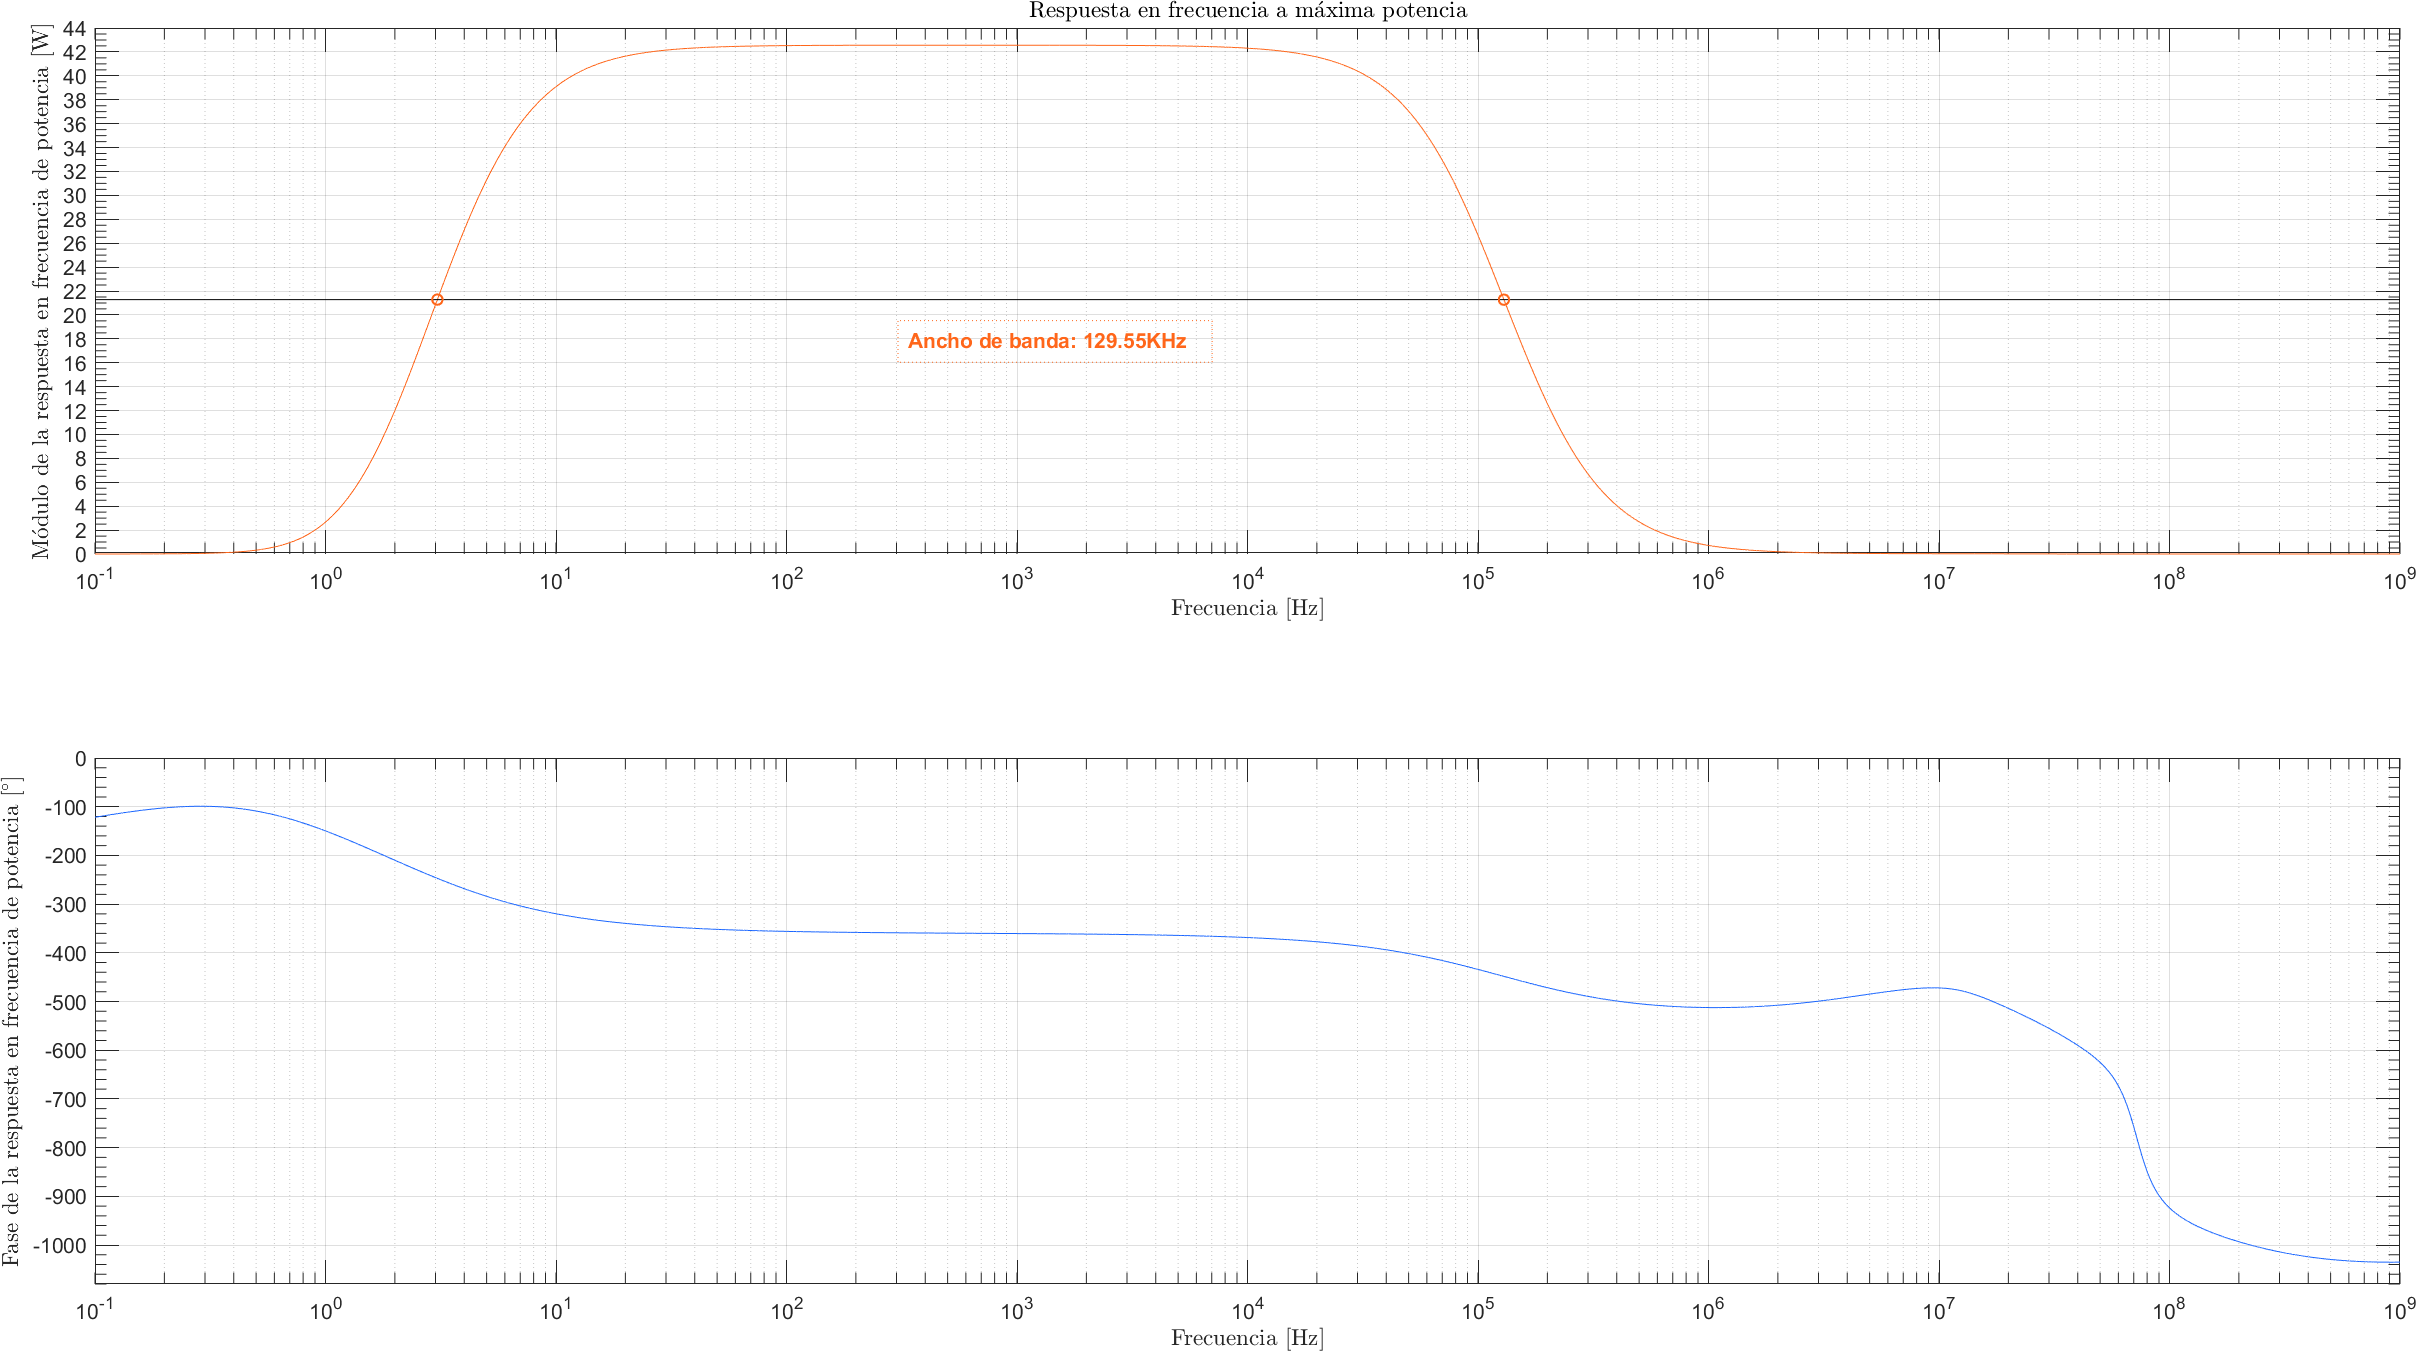
\includegraphics[width=0.9 \textwidth, angle=90]{./img/puntos/P11e_Power_BW.png}
\caption{\label{fig:fig_RF_MAX_POWER}\footnotesize{Respuesta en frecuencia para máxima potencia sobre la carga.}}
\end{center}
\end{figure}


\clearpage

\subsubsection{Respuesta al escalón en pequeña señal}

En la figura~\figref{fig:fig_step_small_signal} se muestra lo obtenido al simular para obtener la respuesta al escalón en pequeña señal, se limitó la salida a un valor de $1 \si[per-mode=symbol]{\volt}$ de pico. La respuesta tiene la forma esperada para un amplificador con acoples capacitivos.

\begin{figure}[H] %htb
\begin{center}
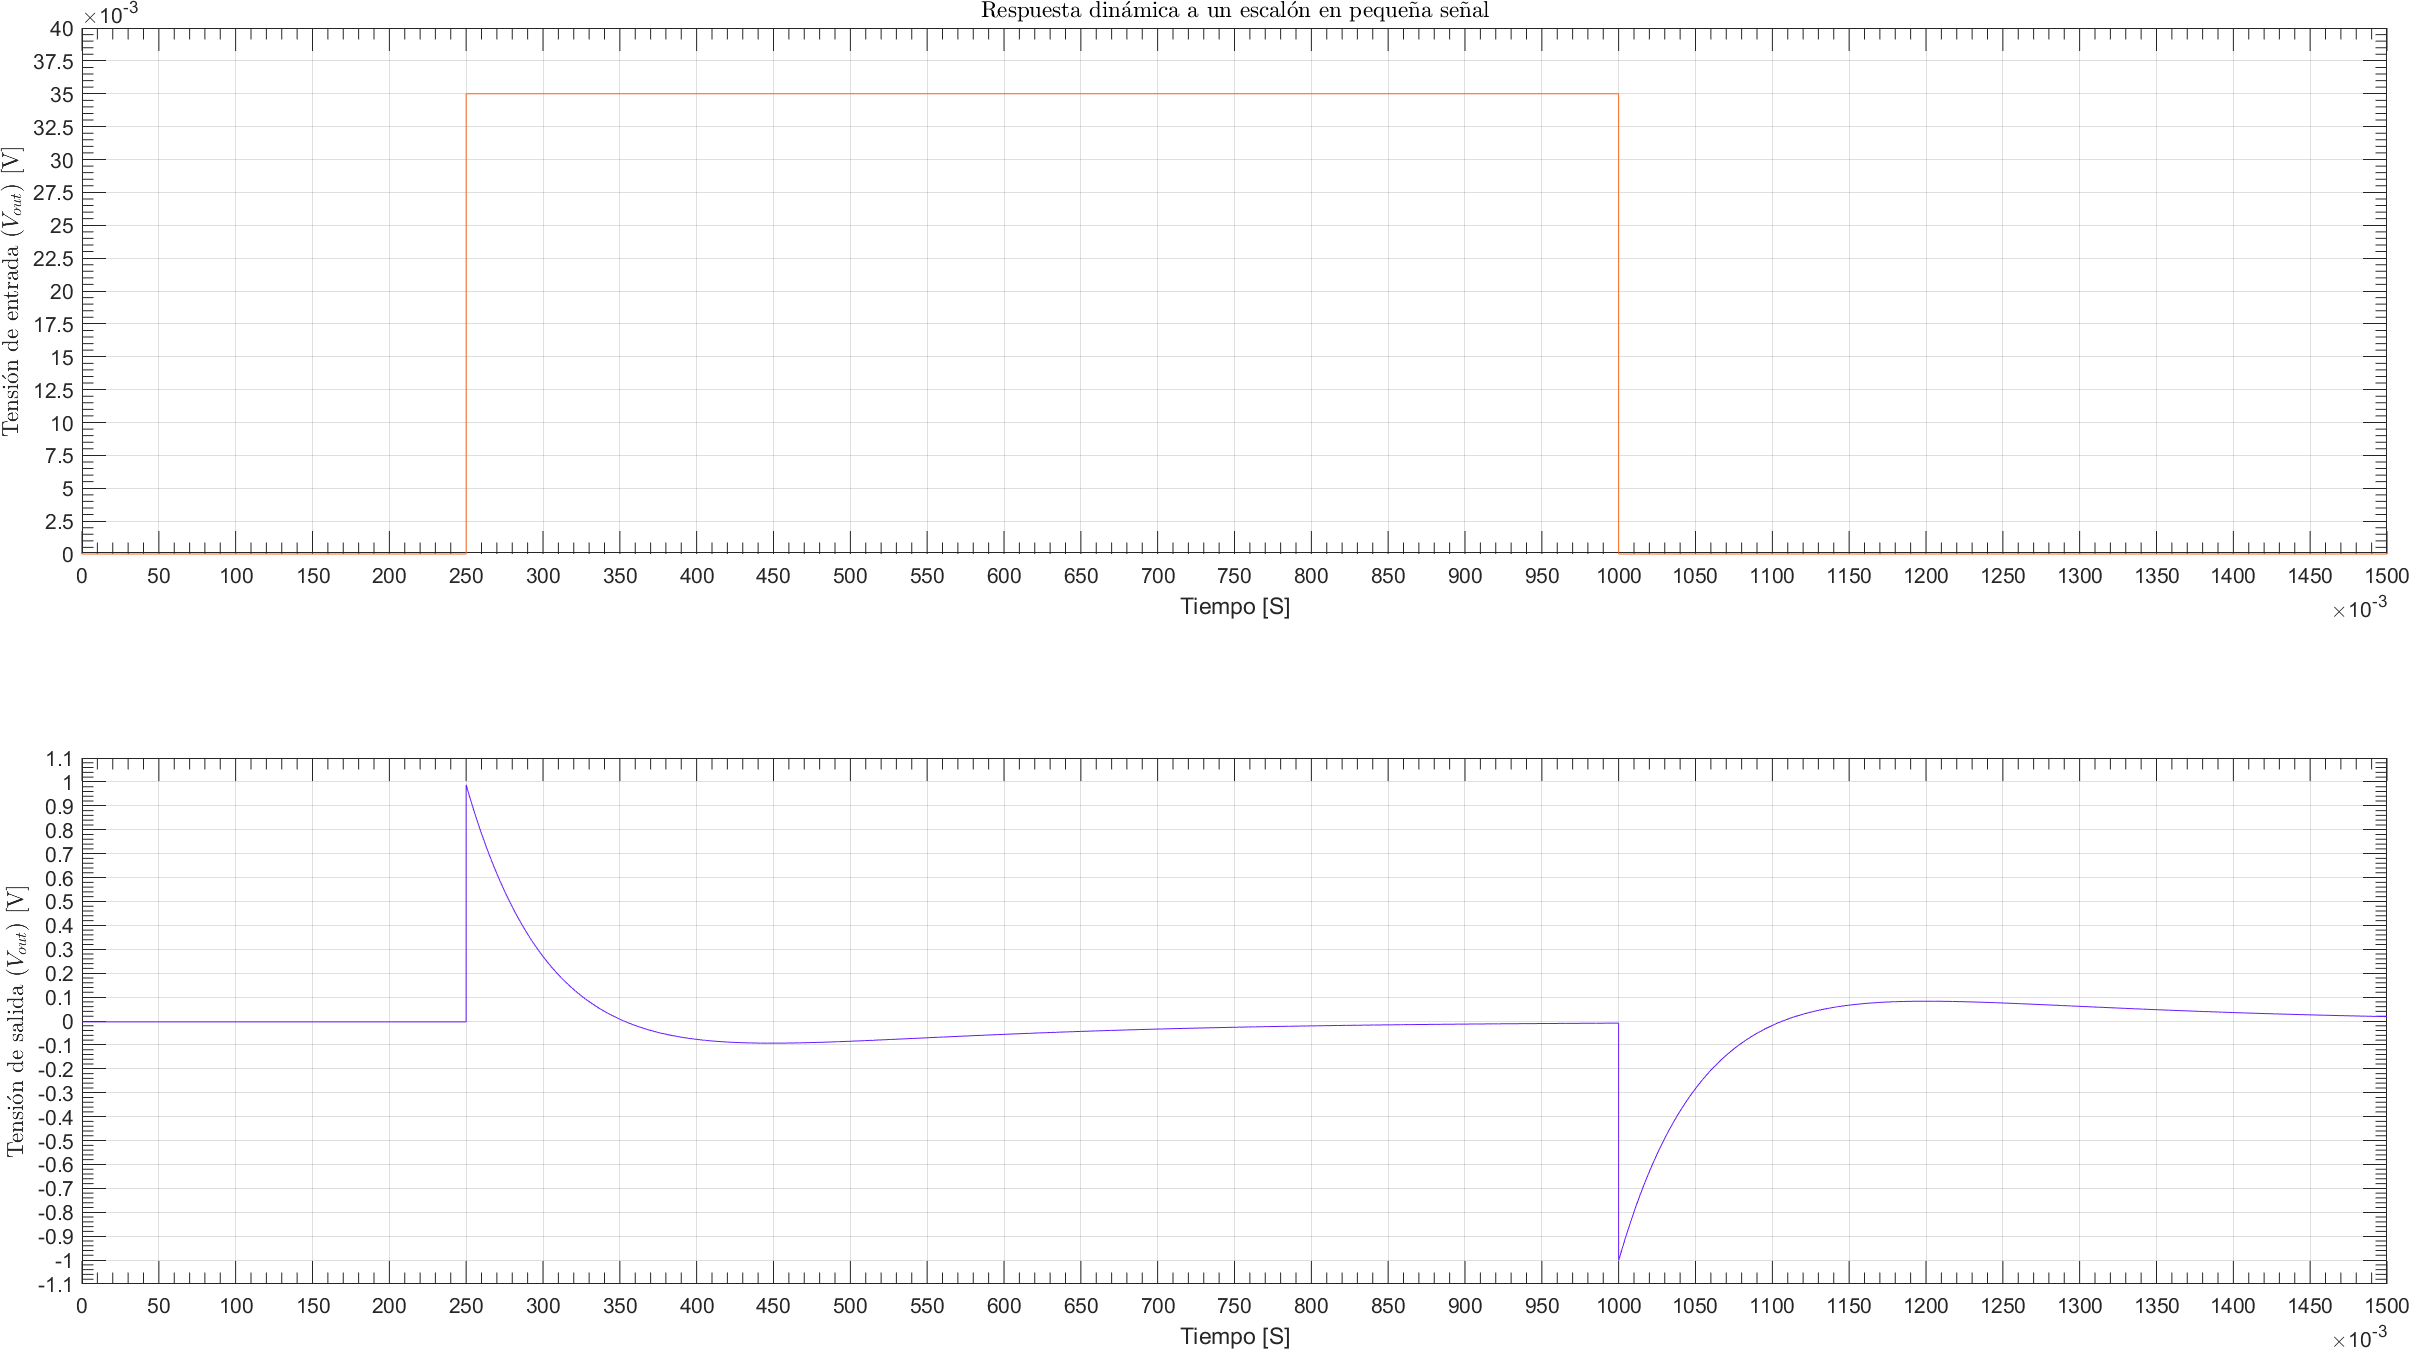
\includegraphics[width=0.9 \textwidth, angle=90]{./img/puntos/P11f_I_step_small_signal.png}
\caption{\label{fig:fig_step_small_signal}\footnotesize{Respuesta al escalón en pequeña señal.}}
\end{center}
\end{figure}


En la figura~\figref{fig:fig_step_small_signal_zoom} se muestra la ampliación del flanco ascendente de la salida, donde se puede apreciar el tiempo de crecimiento, usando la directiva de \textbf{SPICE}, \textit{.measure}, se calculó directamente de la simulación el tiempo de crecimiento entre $10\%$ y $90\%$ y se computó en base a este el ancho de banda del circuito. Se utilizó la expresión que relaciona ancho de banda con el tiempo de crecimiento en un circuito con un solo polo:

\begin{equation}
BW = \frac{0.35}{T_{rise}}
\end{equation}

Se obtuvo:

\begin{equation}
T_{rise} = 2.78 \si[per-mode=symbol]{\micro\second}
\end{equation}


\begin{equation}
\boxed{BW = 125.863 \si[per-mode=symbol]{\kilo\hertz}}
\end{equation}



\begin{figure}[H] %htb
\begin{center}
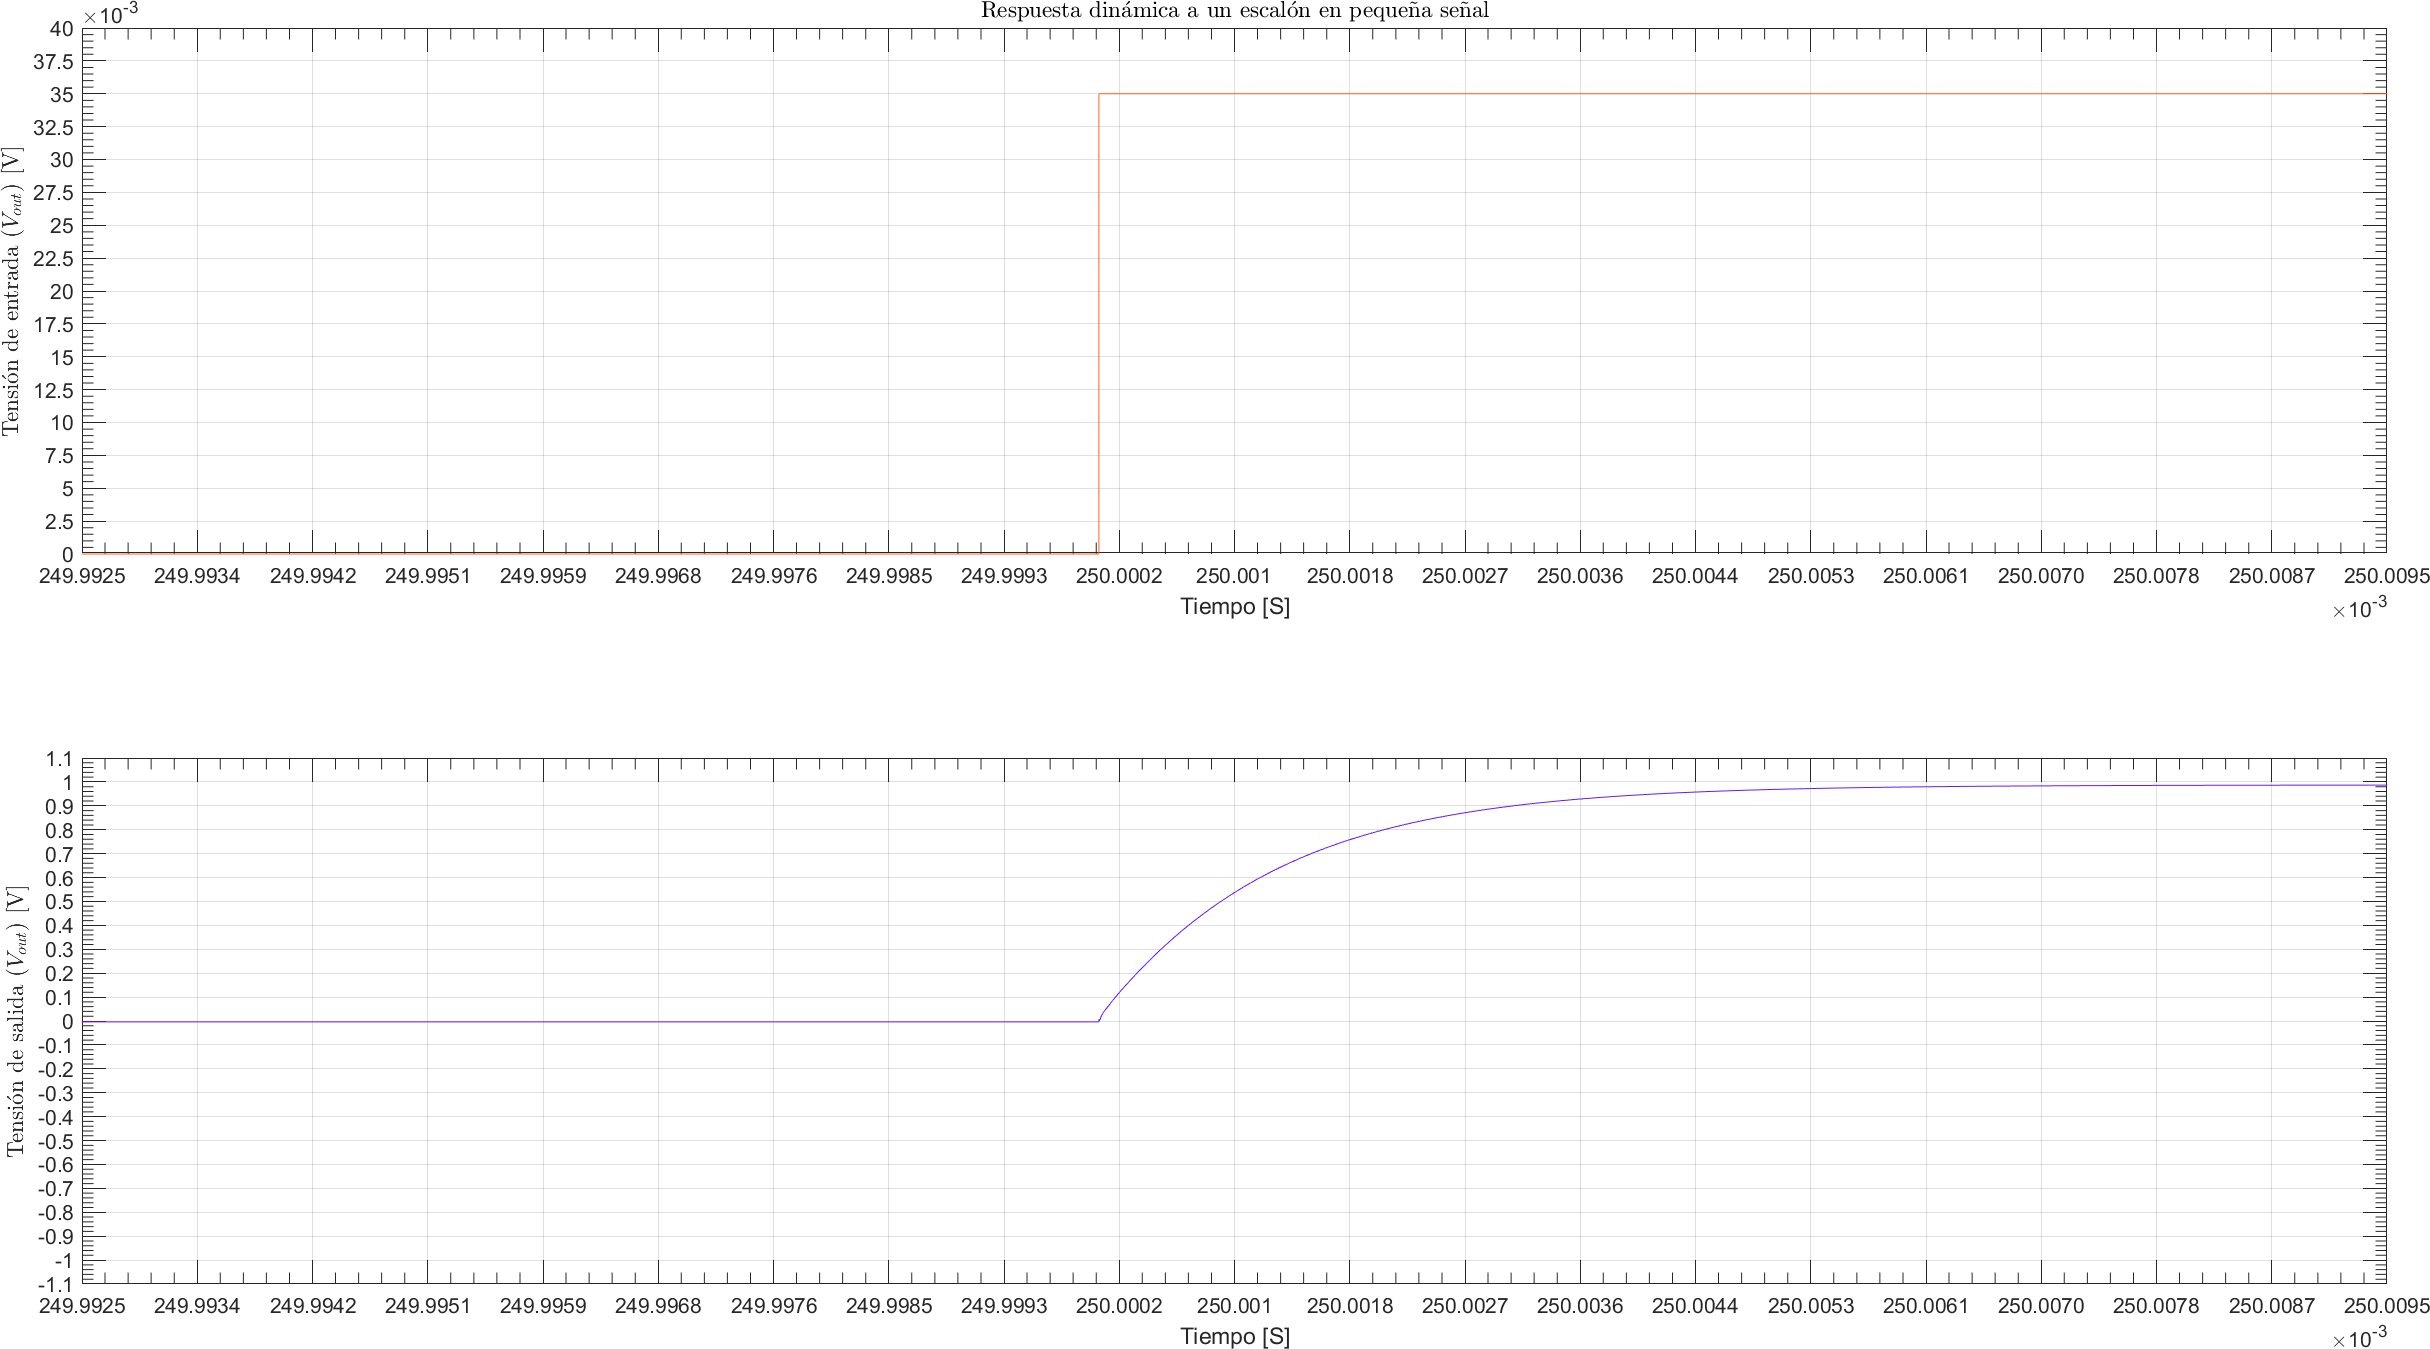
\includegraphics[width=0.9 \textwidth, angle=90]{./img/puntos/P11f_I_step_small_signal_zoom.png}
\caption{\label{fig:fig_step_small_signal_zoom}\footnotesize{Respuesta al escalón en pequeña señal, ampliación del flanco.}}
\end{center}
\end{figure}

\clearpage

\subsubsection{Respuesta al escalón en gran señal}

En la figura~\figref{fig:fig_step_big_signal} se muestra lo obtenido al simular para obtener la respuesta al escalón en gran señal, se llevó la salida a un valor cercano al máximo sin distorsión.

\begin{figure}[H] %htb
\begin{center}
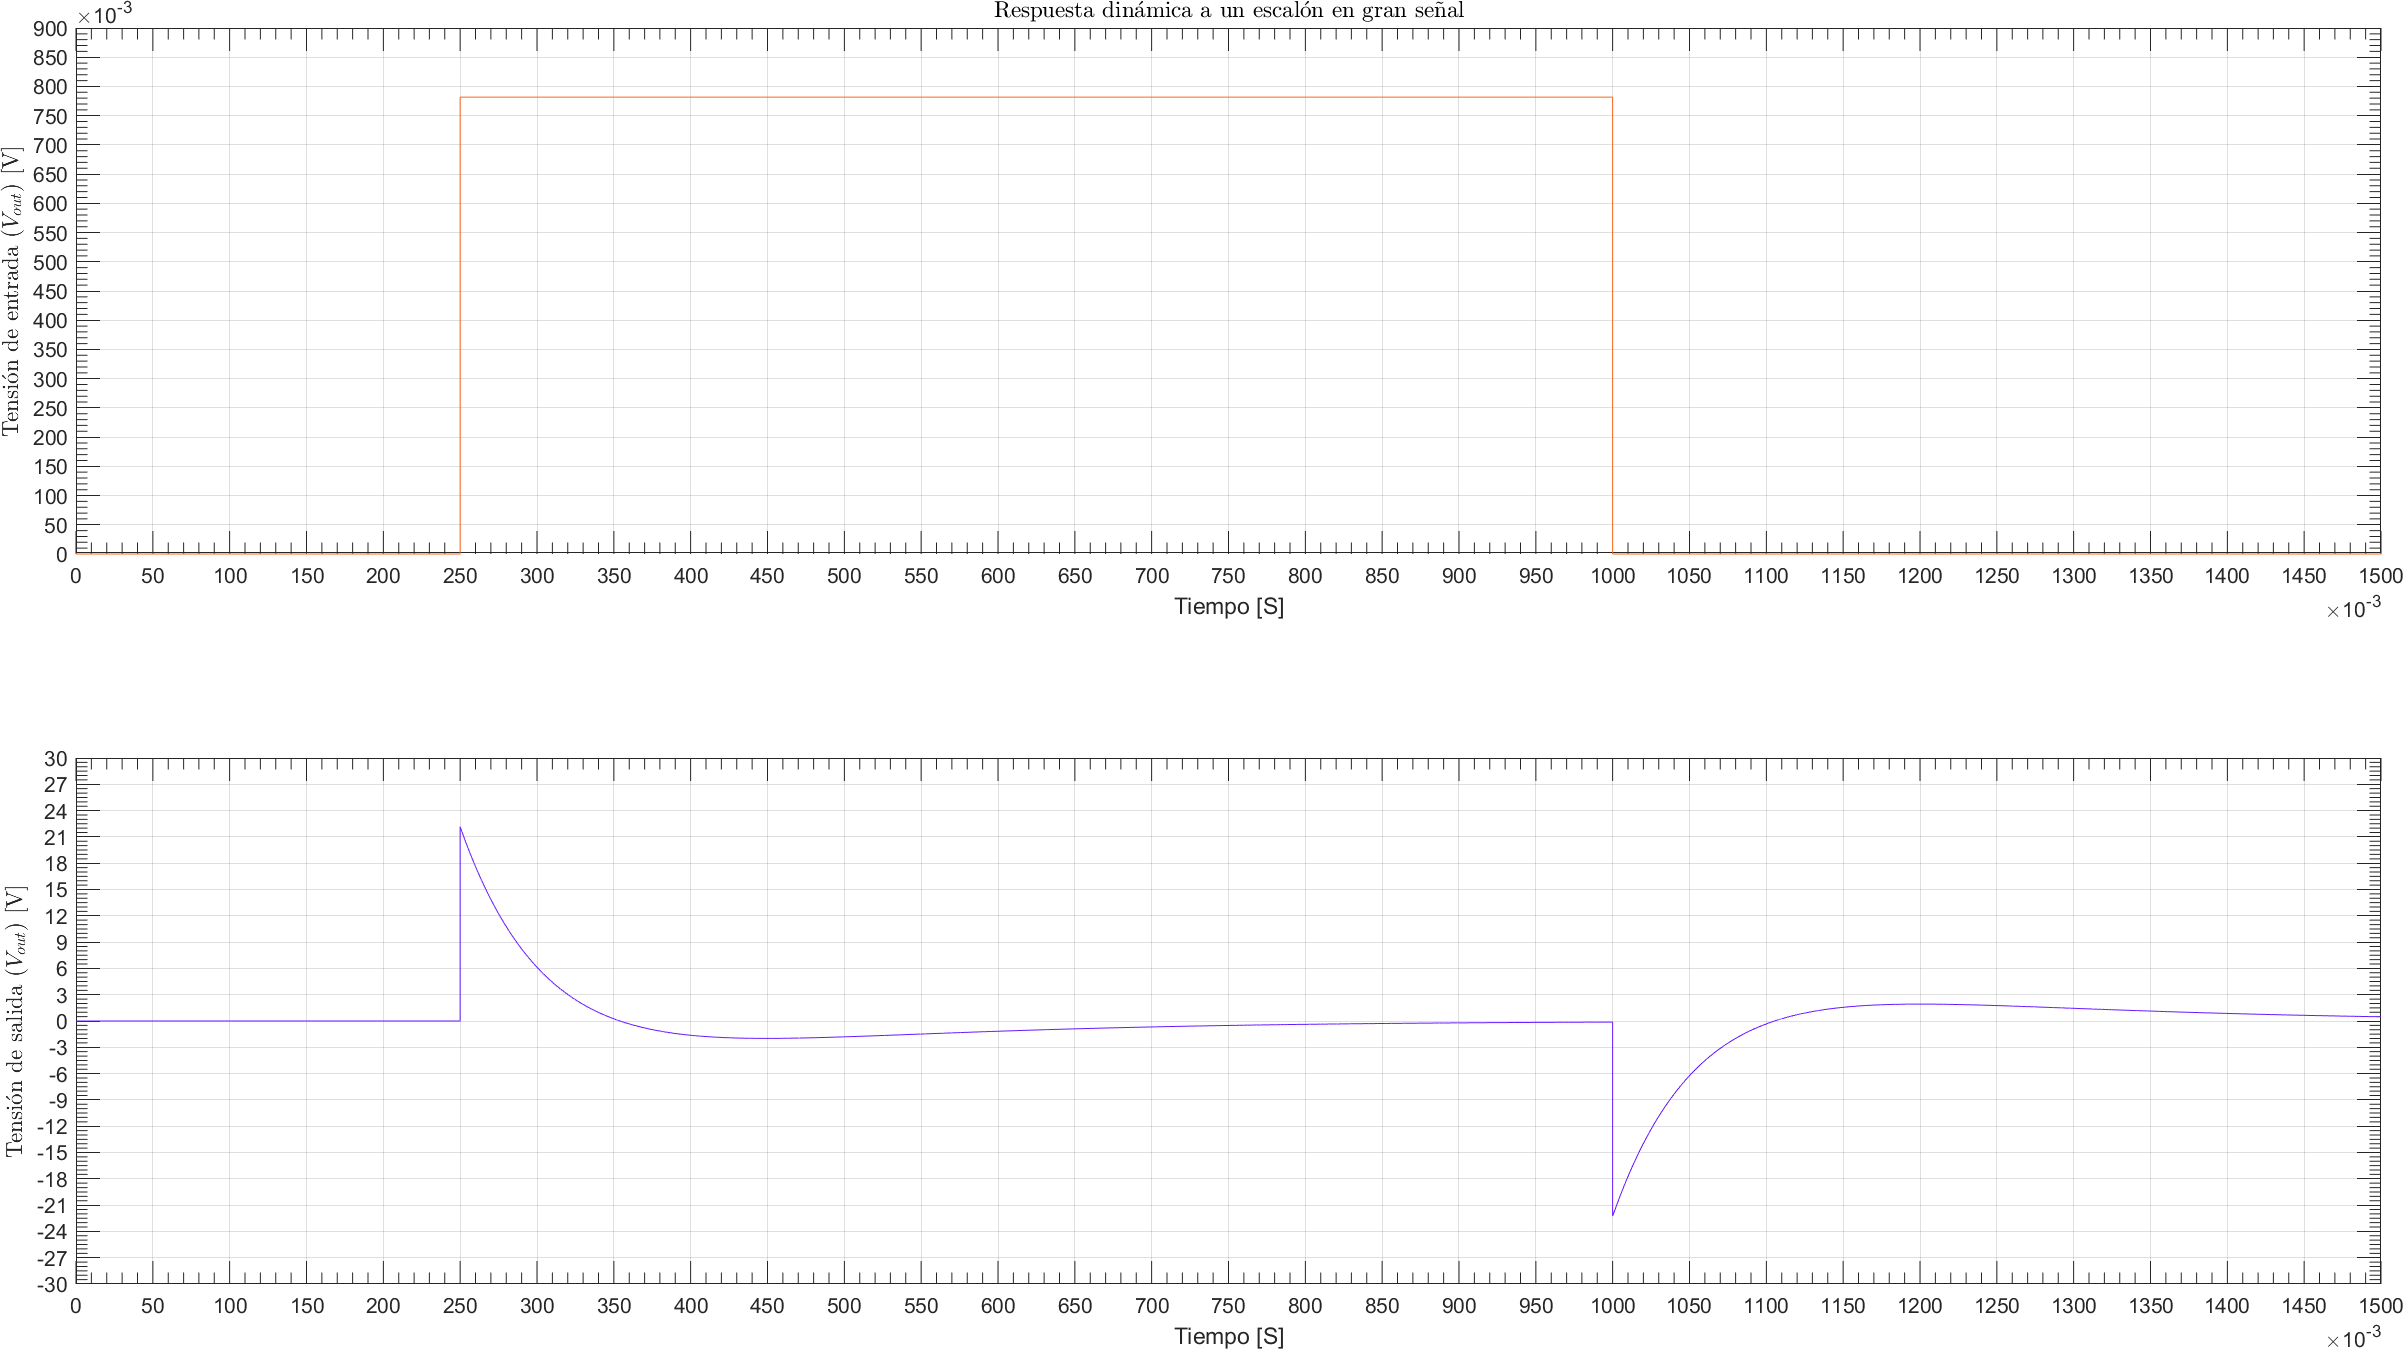
\includegraphics[width=0.9 \textwidth, angle=90]{./img/puntos/P11f_I_step_big_signal.png}
\caption{\label{fig:fig_step_big_signal}\footnotesize{Respuesta al escalón en gran señal.}}
\end{center}
\end{figure}


En la figura~\figref{fig:fig_step_big_signal_zoom} se muestra la ampliación del flanco ascendente de la salida, donde se puede apreciar el tiempo de crecimiento, usando la directiva de \textbf{SPICE}, \textit{.measure}, se calculó directamente de la simulación el \textbf{\quotemarks{slew~rate}}, como la pendiente de subida en el flanco ascendente, se obtuvo:


\begin{equation}
\boxed{SR = 4.39 \si[per-mode=symbol]{\volt\per\micro\second}}
\end{equation}



\begin{figure}[H] %htb
\begin{center}
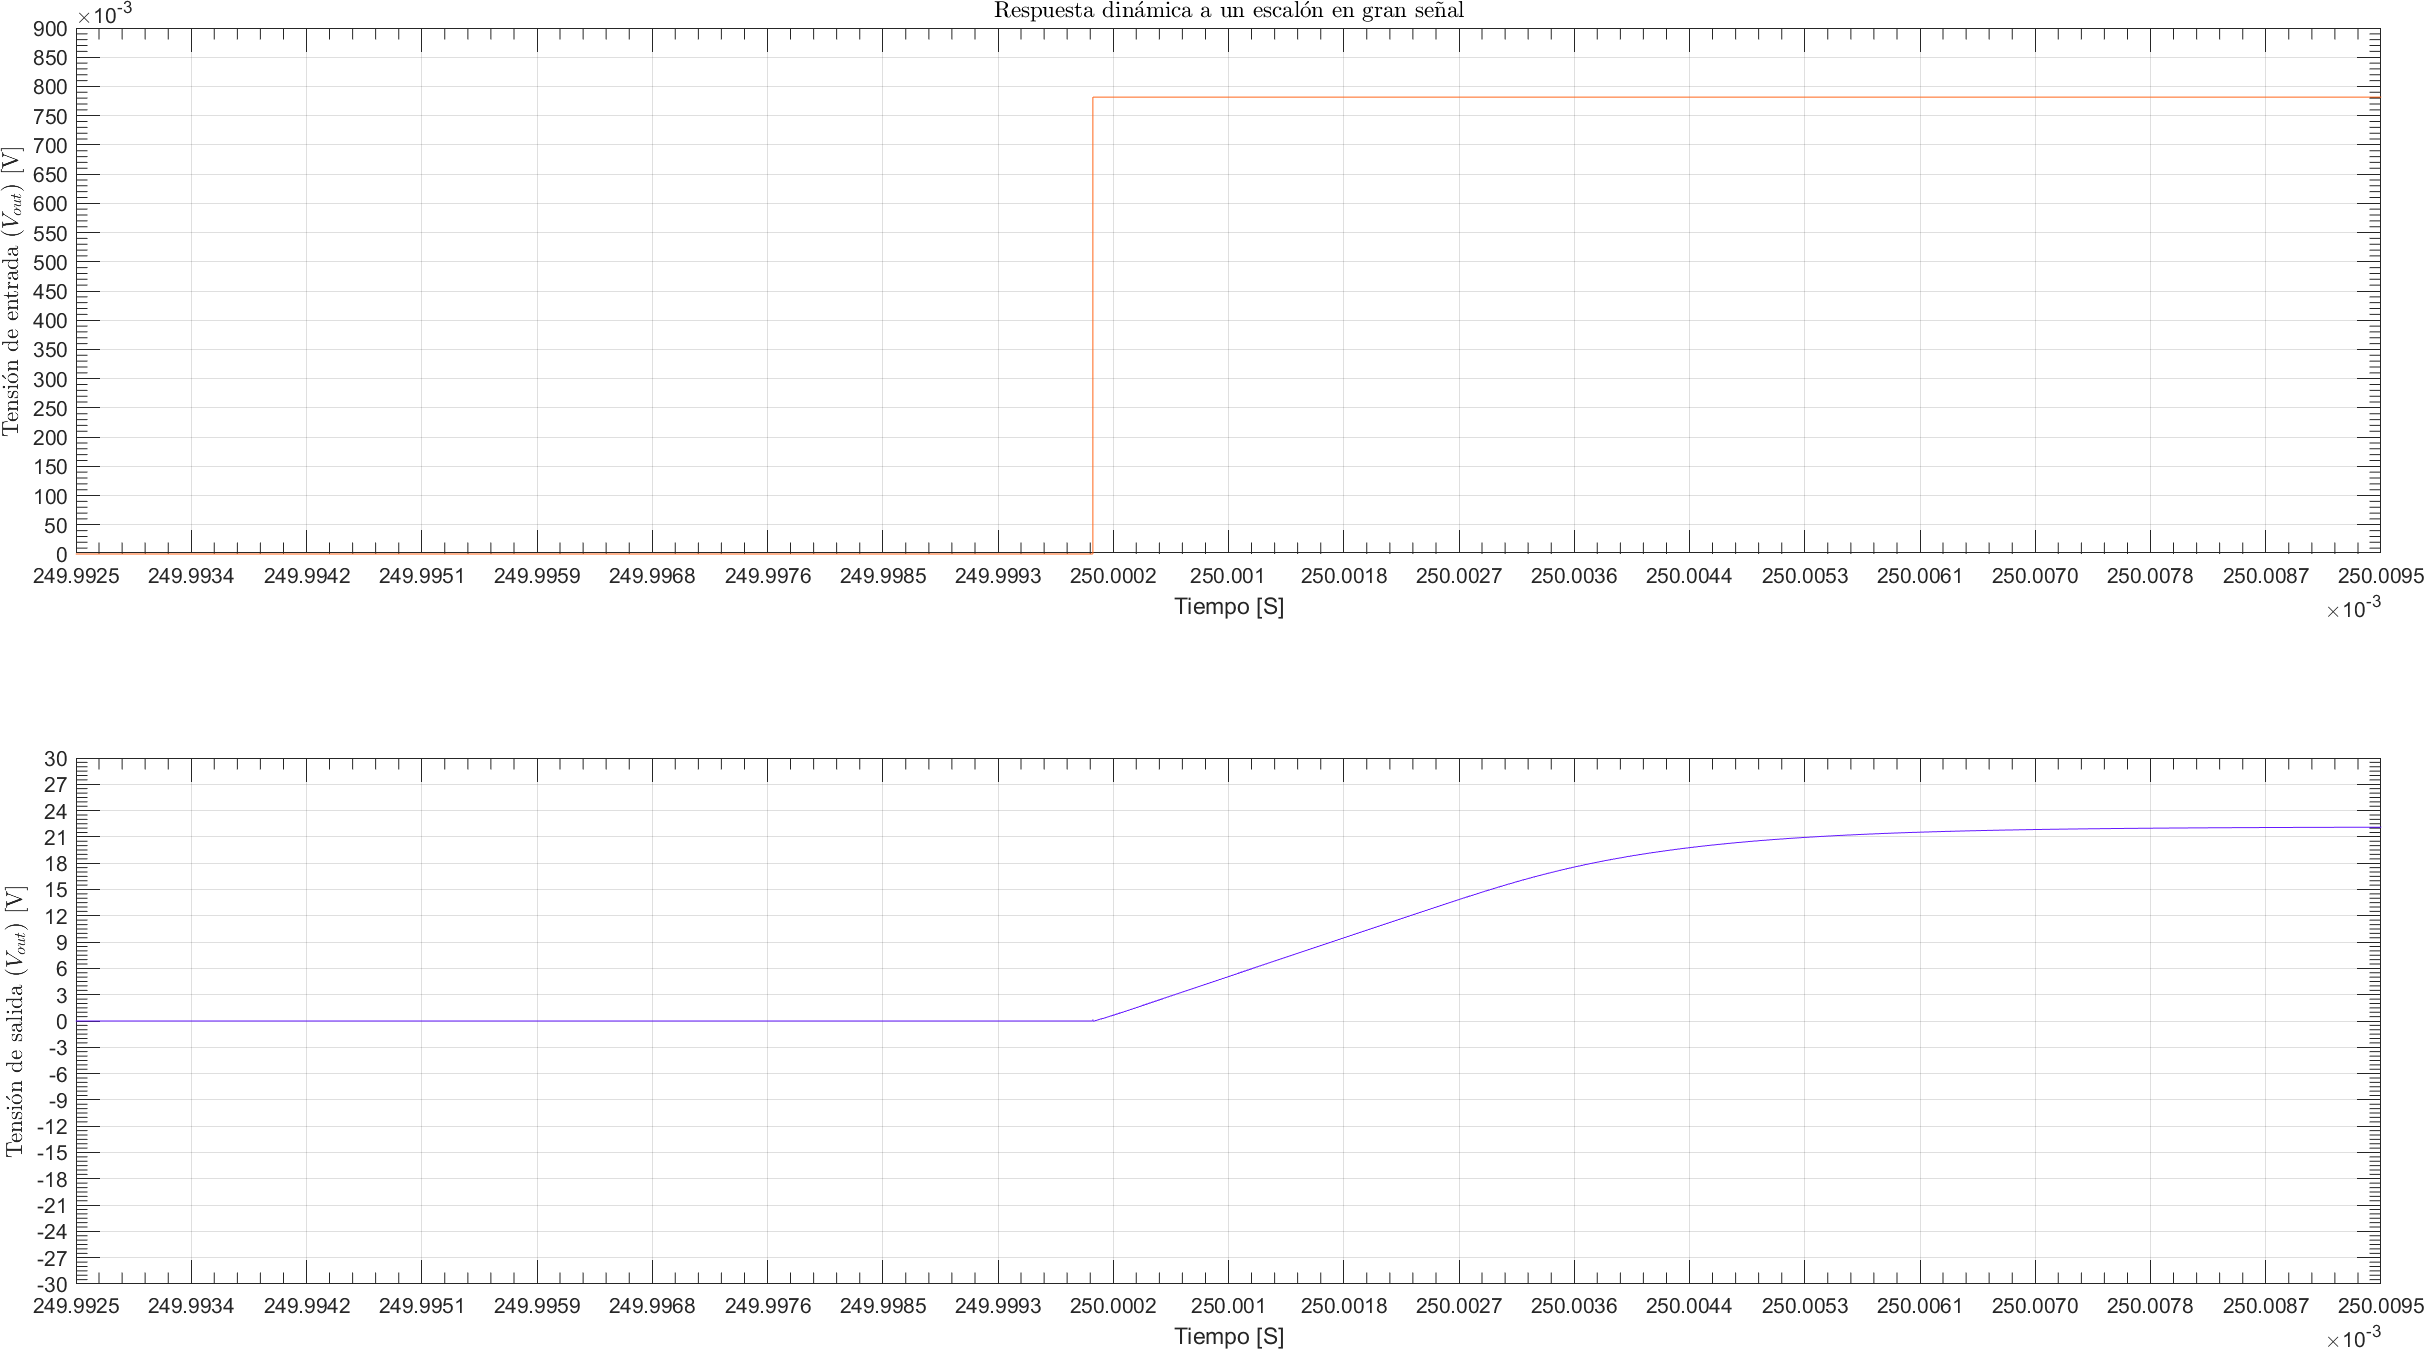
\includegraphics[width=0.9 \textwidth, angle=90]{./img/puntos/P11f_I_step_big_signal_zoom.png}
\caption{\label{fig:fig_step_big_signal_zoom}\footnotesize{Respuesta al escalón en gran señal, ampliación del flanco.}}
\end{center}
\end{figure}

\clearpage


\subsubsection{Margen de fase del amplificador}

En la figura~\figref{fig:fig_phase_margin} se muestra lo obtenido al simular para obtener el margen de fase del circuito, para esta simulación se abrió el lazo de realimentación para la señal y se tomó la respuesta de la cascada del amplificador con la realimentación, en la figura~\figref{fig:fig_loop_gain_circuit}, se puede ver el circuito utilizado para esta simulación. El valor obtenido para el margen de fase es:

\begin{equation}
\boxed{PM = 113.72 \si[per-mode=symbol]{\degree}}
\end{equation}

\begin{figure}[H] %htb
\begin{center}
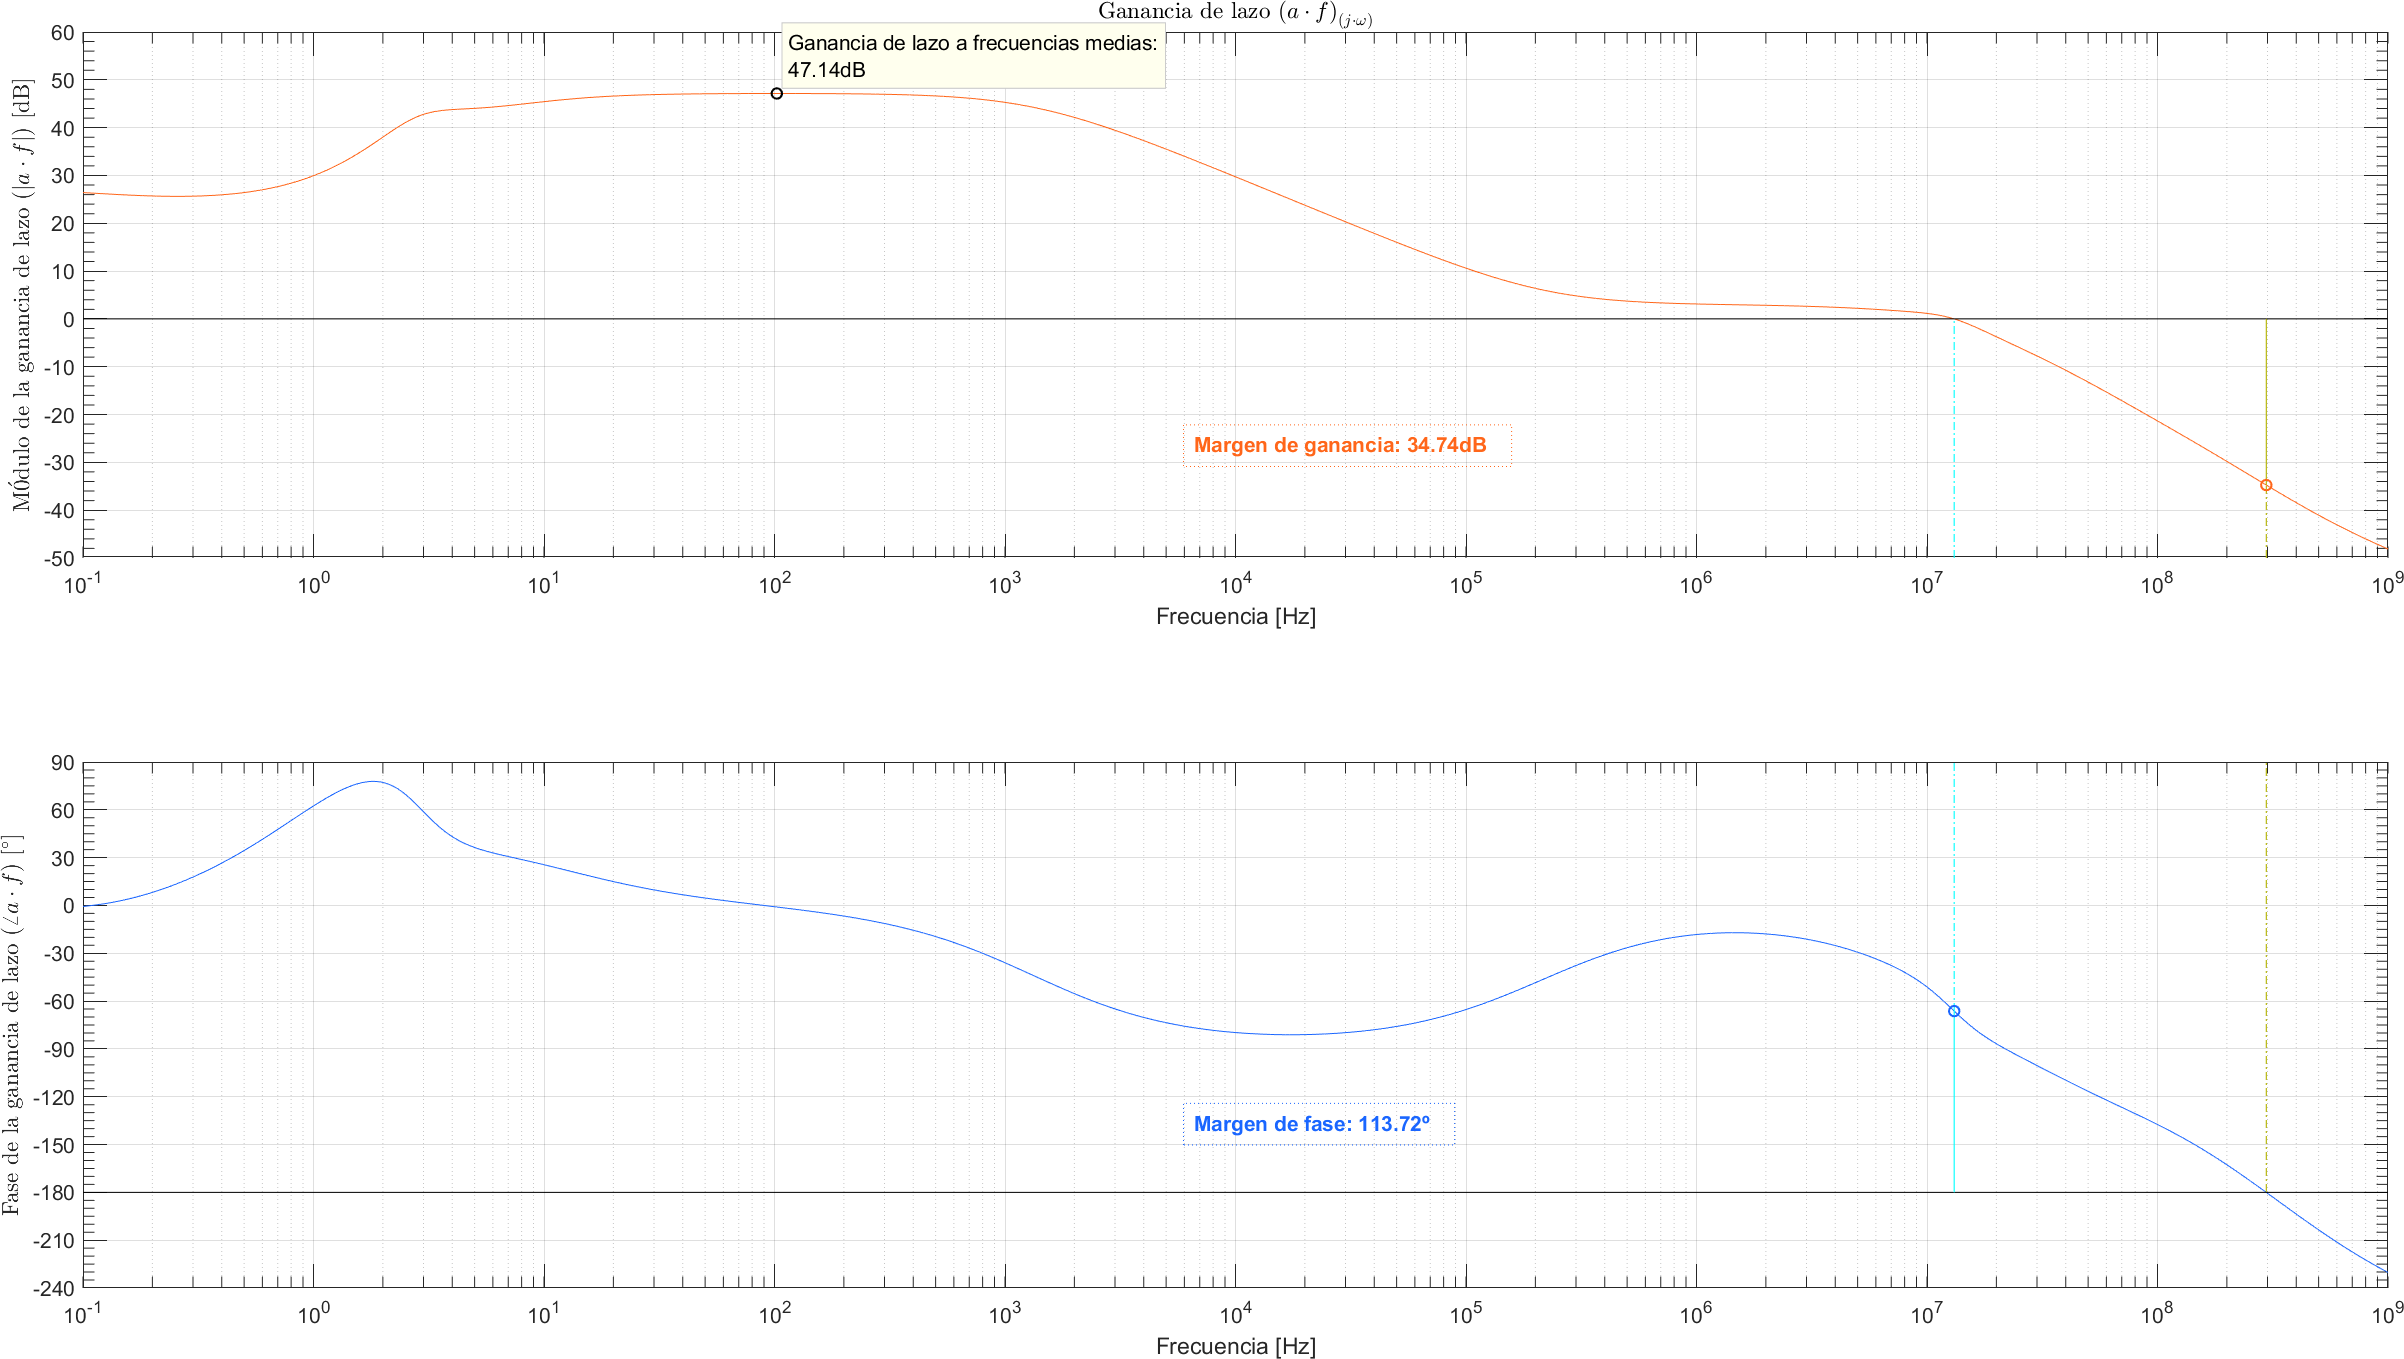
\includegraphics[width=0.9 \textwidth, angle=90]{./img/puntos/P11g_phase_margin.png}
\caption{\label{fig:fig_phase_margin}\footnotesize{Margen de fase.}}
\end{center}
\end{figure}

\begin{figure}[H] %htb
\begin{center}
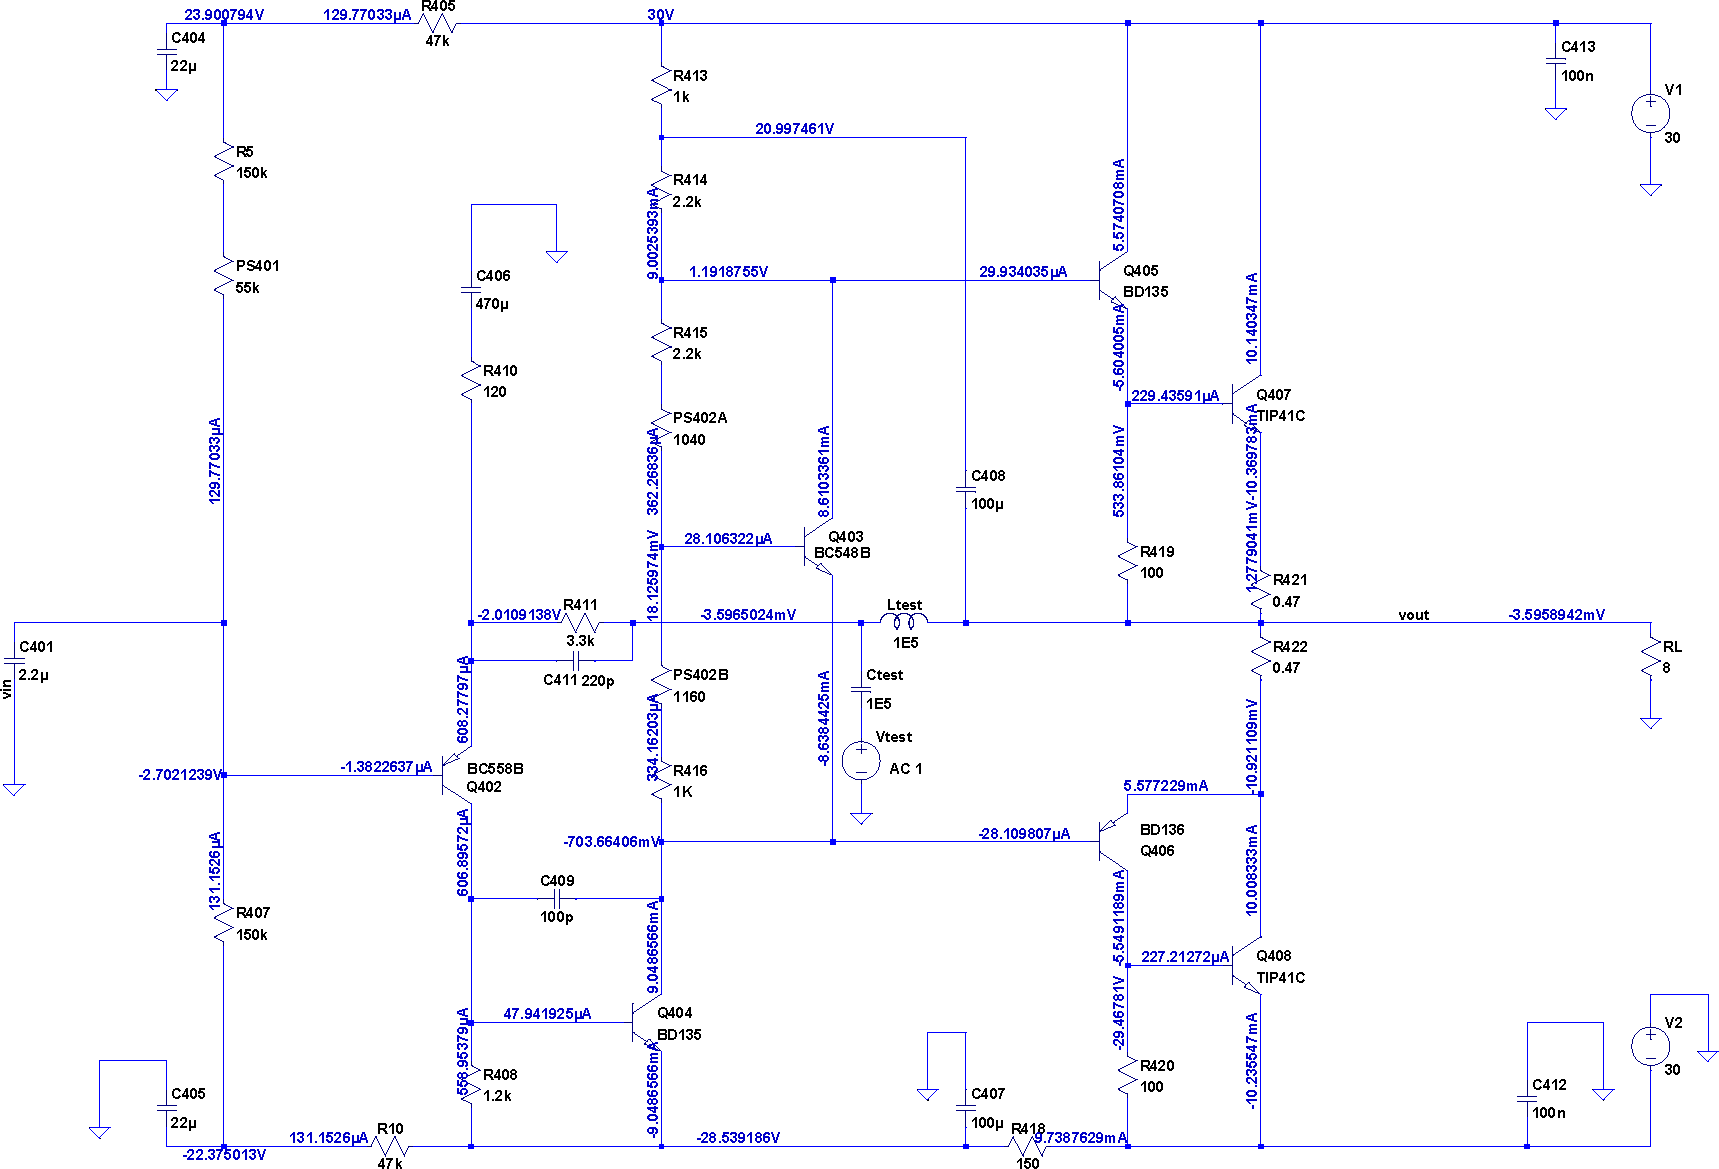
\includegraphics[width=0.9 \textwidth, angle=90]{./img/circuitos_usados/P11g_phase_margin.png}
\caption{\label{fig:fig_loop_gain_circuit}\footnotesize{Circuito usado para simular la ganancia de lazo.}}
\end{center}
\end{figure}

\clearpage

\subsubsection{Distorsión armónica del amplificador}

En el cuadro~\tableref{table:table_THD} se resumen los resultados obtenidos al realizar la simulación para determinar la distorsión armónica total (\textbf{THD}) para 8 combinaciones de frecuencia y potencia de salida sobre la carga. El cálculo se realizo directamente con el comando \textbf{SPICE} \textit{.fourier}, teniendo en cuenta nueve armónicas de la señal y usando todos los datos de aproximadamente $1\si[per-mode=symbol]{\second}$ de simulación.



%% \noindent
%% \begin{center}
 
%%\begin{spacing}{1}  
\begin{table}[H]  %%\centering
    
    \setlength\arrayrulewidth{1.5pt}
    \arrayrulecolor{white}
    \def\clinecolor{\hhline{|>{\arrayrulecolor{white}}-%
    >{\arrayrulecolor{white}}|-|-|-|-|}}
\resizebox{0.8 \textwidth}{!}{% 
       
\begin{tabularx}{1 \textwidth}%
    {|
    >{\columncolor{white} \centering\arraybackslash}m{0.32\linewidth}
     |
    >{\columncolor{white} \centering\arraybackslash}m{0.17\linewidth}
     |
    >{\columncolor{white} \centering\arraybackslash}m{0.17\linewidth}
     |
    >{\columncolor{white} \centering\arraybackslash}m{0.17\linewidth}
     |
    >{\columncolor{white} \centering\arraybackslash}m{0.17\linewidth}
     |
    }
    \rowcolor{HeadersColor} \cellcolor{white} \thead{}  & \thead{$0.1 \si[per-mode=symbol]{\watt}$} & \thead{$1 \si[per-mode=symbol]{\watt}$} & \thead{$10 \si[per-mode=symbol]{\watt}$} & \thead{$90 \%$ de max.} \\    
    \hhline{|-|-|-|-|}
    \rowcolor{gray!20} \cellcolor{HeadersColor} \color{white} $1 \si[per-mode=symbol]{\kilo\hertz}$ & $0.055\%$ & $0.023\%$ & $0.014\%$ & $0.055\%$  \\
    \hhline{|-|-|-|-|}
    \rowcolor{gray!20} \cellcolor{HeadersColor} \color{white} $10 \si[per-mode=symbol]{\kilo\hertz}$ & $0.144\%$ & $0.077\%$ & $0.057\%$ & $0.107\%$   \\
    \hhline{|-|-|-|-|}       
    \end{tabularx}}
	\caption{\footnotesize{Distorsión armónica total (\textbf{THD}).}}
	\label{table:table_THD}
\end{table}
%%\end{spacing}

%% \end{center}

Vemos que la distorsión es menor para $1 \si[per-mode=symbol]{\kilo\hertz}$  de frecuencia de entrada y también que presenta un mínimo alrededor de las potencias medias, es decir, disminuye de bajas a medias potencias y sube de medias a altas potencias.


\clearpage

\subsubsection{Distorsión por intermodulación del amplificador}

En el cuadro~\tableref{table:table_IMD} se resumen los resultados obtenidos al realizar la simulación para determinar la distorsión por intermodulación (\textbf{IMD}) para 4 potencias de salida sobre la carga. El cálculo se realizo con el comando \textbf{SPICE} \textit{.fourier}, se tomaron las armónicas de $100 \si[per-mode=symbol]{\hertz}$ hasta la armónica $55$, de modo de tomar $5$ armónicas por arriba y $5$ armónicas por debajo del tono puro de $5 \si[per-mode=symbol]{\kilo\hertz}$ , y usando todos los datos de aproximadamente $1\si[per-mode=symbol]{\second}$ de simulación.\\
Se observa que la \textbf{IMD} parece crecer para valores bajos y altos de la potencia de salida, teniendo un mínimo a potencias medias.



%% \noindent
%% \begin{center}
 
%%\begin{spacing}{1}  
\begin{table}[H]  %%\centering
    
    \setlength\arrayrulewidth{1.5pt}
    \arrayrulecolor{white}
    \def\clinecolor{\hhline{|>{\arrayrulecolor{white}}-%
    >{\arrayrulecolor{white}}|-|-|-|-|}}
\resizebox{0.8 \textwidth}{!}{% 
       
\begin{tabularx}{1 \textwidth}%
    {|
    >{\columncolor{white} \centering\arraybackslash}m{0.32\linewidth}
     |
    >{\columncolor{white} \centering\arraybackslash}m{0.17\linewidth}
     |
    >{\columncolor{white} \centering\arraybackslash}m{0.17\linewidth}
     |
    >{\columncolor{white} \centering\arraybackslash}m{0.17\linewidth}
     |
    >{\columncolor{white} \centering\arraybackslash}m{0.17\linewidth}
     |
    }
    \rowcolor{HeadersColor} \cellcolor{white} \thead{}  & \thead{$0.1 \si[per-mode=symbol]{\watt}$} & \thead{$1 \si[per-mode=symbol]{\watt}$} & \thead{$10 \si[per-mode=symbol]{\watt}$} & \thead{$90 \%$ de max.} \\    
    \hhline{|-|-|-|-|}
    \rowcolor{gray!20} \cellcolor{HeadersColor} \color{white} \textbf{IMD} & $0.108 \%$ & $0.043 \%$ & $0.048 \%$ & $0.51 \%$ \\
    \hhline{|-|-|-|-|}     
    \end{tabularx}}
	\caption{\footnotesize{Distorsión armónica total (\textbf{IMD}).}}
	\label{table:table_IMD}
\end{table}
%%\end{spacing}

%% \end{center}



\clearpage

\subsubsection{Rechazo de Ruido de la Fuente de Alimentación (\textbf{\quotemarks{PSNR}}).}

En el cuadro~\tableref{table:table_PSNR} se resumen los resultados obtenidos al realizar la simulación para determinar el rechazo de ruido de la fuente de alimentación (\textbf{PSNR}) para 4 frecuencias de la señal de ruido presente en la fuente de alimentación y para una tensión de pico de ruido de $1 \si[per-mode=symbol]{\milli\volt}$.



%% \noindent
%% \begin{center}
 
%%\begin{spacing}{1}  
\begin{table}[H]  %%\centering
    
    \setlength\arrayrulewidth{1.5pt}
    \arrayrulecolor{white}
    \def\clinecolor{\hhline{|>{\arrayrulecolor{white}}-%
    >{\arrayrulecolor{white}}|-|-|-|-|-|-|}}
\resizebox{0.8 \textwidth}{!}{% 
       
\begin{tabularx}{1 \textwidth}%
    {|
    >{\columncolor{white} \centering\arraybackslash}m{0.25\linewidth}
     |
    >{\columncolor{white} \centering\arraybackslash}m{0.125\linewidth}
     |
    >{\columncolor{white} \centering\arraybackslash}m{0.125\linewidth}
     |
    >{\columncolor{white} \centering\arraybackslash}m{0.125\linewidth}
     |
    >{\columncolor{white} \centering\arraybackslash}m{0.125\linewidth}
     |
    >{\columncolor{white} \centering\arraybackslash}m{0.125\linewidth}
     |
    >{\columncolor{white} \centering\arraybackslash}m{0.125\linewidth}
     |
    }
    \rowcolor{HeadersColor} \cellcolor{white} \thead{}  & \thead{$50 \si[per-mode=symbol]{\hertz}$} & \thead{$100 \si[per-mode=symbol]{\hertz}$} & \thead{$1 \si[per-mode=symbol]{\kilo\hertz}$} & \thead{ $10 \si[per-mode=symbol]{\kilo\hertz}$} & \thead{$50 \si[per-mode=symbol]{\kilo\hertz}$} & \thead{$100 \si[per-mode=symbol]{\kilo\hertz}$}\\    
    \hhline{|-|-|-|-|-|-|}
    \rowcolor{gray!20} \cellcolor{HeadersColor} \color{white} \textbf{PSNR} & $ 53.2 \si[per-mode=symbol]{\decibel} $ & $ 59.1 \si[per-mode=symbol]{\decibel} $ & $ 78.99 \si[per-mode=symbol]{\decibel} $ & $ 93.07 \si[per-mode=symbol]{\decibel} $ & $ 89.18 \si[per-mode=symbol]{\decibel} $ & $ 84.82 \si[per-mode=symbol]{\decibel} $ \\
    \hhline{|-|-|-|-|-|-|}     
    \end{tabularx}}
	\caption{\footnotesize{Rechazo de Ruido de la Fuente de Alimentación (\textbf{\quotemarks{PSNR}}).}}
	\label{table:table_PSNR}
\end{table}
%%\end{spacing}

%% \end{center}

El rechazo al ruido de la fuente parece ser mayor cerca del centro de la banda del amplificador.

